\documentclass[twoside]{book}

% Packages required by doxygen
\usepackage{fixltx2e}
\usepackage{calc}
\usepackage{doxygen}
\usepackage[export]{adjustbox} % also loads graphicx
\usepackage{graphicx}
\usepackage[utf8]{inputenc}
\usepackage{makeidx}
\usepackage{multicol}
\usepackage{multirow}
\PassOptionsToPackage{warn}{textcomp}
\usepackage{textcomp}
\usepackage[nointegrals]{wasysym}
\usepackage[table]{xcolor}

% Font selection
\usepackage[T1]{fontenc}
\usepackage[scaled=.90]{helvet}
\usepackage{courier}
\usepackage{amssymb}
\usepackage{sectsty}
\renewcommand{\familydefault}{\sfdefault}
\allsectionsfont{%
  \fontseries{bc}\selectfont%
  \color{darkgray}%
}
\renewcommand{\DoxyLabelFont}{%
  \fontseries{bc}\selectfont%
  \color{darkgray}%
}
\newcommand{\+}{\discretionary{\mbox{\scriptsize$\hookleftarrow$}}{}{}}

% Page & text layout
\usepackage{geometry}
\geometry{%
  a4paper,%
  top=2.5cm,%
  bottom=2.5cm,%
  left=2.5cm,%
  right=2.5cm%
}
\tolerance=750
\hfuzz=15pt
\hbadness=750
\setlength{\emergencystretch}{15pt}
\setlength{\parindent}{0cm}
\setlength{\parskip}{3ex plus 2ex minus 2ex}
\makeatletter
\renewcommand{\paragraph}{%
  \@startsection{paragraph}{4}{0ex}{-1.0ex}{1.0ex}{%
    \normalfont\normalsize\bfseries\SS@parafont%
  }%
}
\renewcommand{\subparagraph}{%
  \@startsection{subparagraph}{5}{0ex}{-1.0ex}{1.0ex}{%
    \normalfont\normalsize\bfseries\SS@subparafont%
  }%
}
\makeatother

% Headers & footers
\usepackage{fancyhdr}
\pagestyle{fancyplain}
\fancyhead[LE]{\fancyplain{}{\bfseries\thepage}}
\fancyhead[CE]{\fancyplain{}{}}
\fancyhead[RE]{\fancyplain{}{\bfseries\leftmark}}
\fancyhead[LO]{\fancyplain{}{\bfseries\rightmark}}
\fancyhead[CO]{\fancyplain{}{}}
\fancyhead[RO]{\fancyplain{}{\bfseries\thepage}}
\fancyfoot[LE]{\fancyplain{}{}}
\fancyfoot[CE]{\fancyplain{}{}}
\fancyfoot[RE]{\fancyplain{}{\bfseries\scriptsize Generated by Doxygen }}
\fancyfoot[LO]{\fancyplain{}{\bfseries\scriptsize Generated by Doxygen }}
\fancyfoot[CO]{\fancyplain{}{}}
\fancyfoot[RO]{\fancyplain{}{}}
\renewcommand{\footrulewidth}{0.4pt}
\renewcommand{\chaptermark}[1]{%
  \markboth{#1}{}%
}
\renewcommand{\sectionmark}[1]{%
  \markright{\thesection\ #1}%
}

% Indices & bibliography
\usepackage{natbib}
\usepackage[titles]{tocloft}
\setcounter{tocdepth}{3}
\setcounter{secnumdepth}{5}
\makeindex

% Hyperlinks (required, but should be loaded last)
\usepackage{ifpdf}
\ifpdf
  \usepackage[pdftex,pagebackref=true]{hyperref}
\else
  \usepackage[ps2pdf,pagebackref=true]{hyperref}
\fi
\hypersetup{%
  colorlinks=true,%
  linkcolor=blue,%
  citecolor=blue,%
  unicode%
}

% Custom commands
\newcommand{\clearemptydoublepage}{%
  \newpage{\pagestyle{empty}\cleardoublepage}%
}

\usepackage{caption}
\captionsetup{labelsep=space,justification=centering,font={bf},singlelinecheck=off,skip=4pt,position=top}

%===== C O N T E N T S =====

\begin{document}

% Titlepage & ToC
\hypersetup{pageanchor=false,
             bookmarksnumbered=true,
             pdfencoding=unicode
            }
\pagenumbering{alph}
\begin{titlepage}
\vspace*{7cm}
\begin{center}%
{\Large Mvc \\[1ex]\large 1.\+0 }\\
\vspace*{1cm}
{\large Generated by Doxygen 1.8.13}\\
\end{center}
\end{titlepage}
\clearemptydoublepage
\pagenumbering{roman}
\tableofcontents
\clearemptydoublepage
\pagenumbering{arabic}
\hypersetup{pageanchor=true}

%--- Begin generated contents ---
\chapter{Namespace Index}
\section{Packages}
Here are the packages with brief descriptions (if available)\+:\begin{DoxyCompactList}
\item\contentsline{section}{\hyperlink{namespace_mvc}{Mvc} }{\pageref{namespace_mvc}}{}
\end{DoxyCompactList}

\chapter{Hierarchical Index}
\section{Class Hierarchy}
This inheritance list is sorted roughly, but not completely, alphabetically\+:\begin{DoxyCompactList}
\item Attribute\begin{DoxyCompactList}
\item \contentsline{section}{Mvc.\+Filter\+Attribute}{\pageref{class_mvc_1_1_filter_attribute}}{}
\begin{DoxyCompactList}
\item \contentsline{section}{Mvc.\+Authorize\+Attribute}{\pageref{class_mvc_1_1_authorize_attribute}}{}
\item \contentsline{section}{Mvc.\+Http\+Method}{\pageref{class_mvc_1_1_http_method}}{}
\begin{DoxyCompactList}
\item \contentsline{section}{Mvc.\+Http\+Delete}{\pageref{class_mvc_1_1_http_delete}}{}
\item \contentsline{section}{Mvc.\+Http\+Get}{\pageref{class_mvc_1_1_http_get}}{}
\item \contentsline{section}{Mvc.\+Http\+Post}{\pageref{class_mvc_1_1_http_post}}{}
\item \contentsline{section}{Mvc.\+Http\+Put}{\pageref{class_mvc_1_1_http_put}}{}
\end{DoxyCompactList}
\end{DoxyCompactList}
\end{DoxyCompactList}
\item \contentsline{section}{Mvc.\+Base\+Controller}{\pageref{class_mvc_1_1_base_controller}}{}
\item \contentsline{section}{Mvc.\+Configuration\+Manager}{\pageref{class_mvc_1_1_configuration_manager}}{}
\item \contentsline{section}{Mvc.\+Http\+Context}{\pageref{class_mvc_1_1_http_context}}{}
\item \contentsline{section}{Mvc.\+Http\+File}{\pageref{class_mvc_1_1_http_file}}{}
\item \contentsline{section}{Mvc.\+I\+Action\+Result}{\pageref{interface_mvc_1_1_i_action_result}}{}
\begin{DoxyCompactList}
\item \contentsline{section}{Mvc.\+Content}{\pageref{class_mvc_1_1_content}}{}
\item \contentsline{section}{Mvc.\+Json}{\pageref{class_mvc_1_1_json}}{}
\item \contentsline{section}{Mvc.\+View}{\pageref{class_mvc_1_1_view}}{}
\end{DoxyCompactList}
\item I\+P\+Http\+Application\begin{DoxyCompactList}
\item \contentsline{section}{Mvc.\+P\+Http\+Application}{\pageref{class_mvc_1_1_p_http_application}}{}
\end{DoxyCompactList}
\item \contentsline{section}{Mvc.\+Request}{\pageref{class_mvc_1_1_request}}{}
\item \contentsline{section}{Mvc.\+Route}{\pageref{class_mvc_1_1_route}}{}
\item \contentsline{section}{Mvc.\+Session}{\pageref{class_mvc_1_1_session}}{}
\item \contentsline{section}{Mvc.\+User}{\pageref{class_mvc_1_1_user}}{}
\end{DoxyCompactList}

\chapter{Class Index}
\section{Class List}
Here are the classes, structs, unions and interfaces with brief descriptions\+:\begin{DoxyCompactList}
\item\contentsline{section}{\hyperlink{class_mvc_1_1_authorize_attribute}{Mvc.\+Authorize\+Attribute} \\*Representative class of an authorization attribute for the controllers methods. }{\pageref{class_mvc_1_1_authorize_attribute}}{}
\item\contentsline{section}{\hyperlink{class_mvc_1_1_base_controller}{Mvc.\+Base\+Controller} \\*Representative class of a base controller }{\pageref{class_mvc_1_1_base_controller}}{}
\item\contentsline{section}{\hyperlink{class_mvc_1_1_configuration_manager}{Mvc.\+Configuration\+Manager} \\*Representative class of an app configuration manager. }{\pageref{class_mvc_1_1_configuration_manager}}{}
\item\contentsline{section}{\hyperlink{class_mvc_1_1_content}{Mvc.\+Content} \\*Representative class of a raw content (or redirection) response of a controller }{\pageref{class_mvc_1_1_content}}{}
\item\contentsline{section}{\hyperlink{class_mvc_1_1_filter_attribute}{Mvc.\+Filter\+Attribute} \\*Representative abstract class of a filter attribute. }{\pageref{class_mvc_1_1_filter_attribute}}{}
\item\contentsline{section}{\hyperlink{class_mvc_1_1_http_context}{Mvc.\+Http\+Context} \\*Representative class of the context information of the http server. }{\pageref{class_mvc_1_1_http_context}}{}
\item\contentsline{section}{\hyperlink{class_mvc_1_1_http_delete}{Mvc.\+Http\+Delete} \\*Representative class of and http D\+E\+L\+E\+TE method attribute }{\pageref{class_mvc_1_1_http_delete}}{}
\item\contentsline{section}{\hyperlink{class_mvc_1_1_http_file}{Mvc.\+Http\+File} \\*Representative class of a file comming in an http request. }{\pageref{class_mvc_1_1_http_file}}{}
\item\contentsline{section}{\hyperlink{class_mvc_1_1_http_get}{Mvc.\+Http\+Get} \\*Representative class of and http G\+ET method attribute }{\pageref{class_mvc_1_1_http_get}}{}
\item\contentsline{section}{\hyperlink{class_mvc_1_1_http_method}{Mvc.\+Http\+Method} \\*Representative class of and http method attribute }{\pageref{class_mvc_1_1_http_method}}{}
\item\contentsline{section}{\hyperlink{class_mvc_1_1_http_post}{Mvc.\+Http\+Post} \\*Representative class of and http P\+O\+ST method attribute }{\pageref{class_mvc_1_1_http_post}}{}
\item\contentsline{section}{\hyperlink{class_mvc_1_1_http_put}{Mvc.\+Http\+Put} \\*Representative class of and http P\+UT method attribute }{\pageref{class_mvc_1_1_http_put}}{}
\item\contentsline{section}{\hyperlink{interface_mvc_1_1_i_action_result}{Mvc.\+I\+Action\+Result} \\*Representative interface of the result of a Controller }{\pageref{interface_mvc_1_1_i_action_result}}{}
\item\contentsline{section}{\hyperlink{class_mvc_1_1_json}{Mvc.\+Json} \\*Representative class of a json response }{\pageref{class_mvc_1_1_json}}{}
\item\contentsline{section}{\hyperlink{class_mvc_1_1_p_http_application}{Mvc.\+P\+Http\+Application} \\*Interface of a Http application hosted in our Web Server. }{\pageref{class_mvc_1_1_p_http_application}}{}
\item\contentsline{section}{\hyperlink{class_mvc_1_1_request}{Mvc.\+Request} \\*Representative class of a parsed request }{\pageref{class_mvc_1_1_request}}{}
\item\contentsline{section}{\hyperlink{class_mvc_1_1_route}{Mvc.\+Route} \\*Representative class of a route. }{\pageref{class_mvc_1_1_route}}{}
\item\contentsline{section}{\hyperlink{class_mvc_1_1_session}{Mvc.\+Session} \\*Representative class of the unique application session }{\pageref{class_mvc_1_1_session}}{}
\item\contentsline{section}{\hyperlink{class_mvc_1_1_user}{Mvc.\+User} \\*Representative class of an application basic user. }{\pageref{class_mvc_1_1_user}}{}
\item\contentsline{section}{\hyperlink{class_mvc_1_1_view}{Mvc.\+View} \\*Representative class of a custom view. }{\pageref{class_mvc_1_1_view}}{}
\end{DoxyCompactList}

\chapter{Namespace Documentation}
\hypertarget{namespace_mvc}{}\section{Mvc Namespace Reference}
\label{namespace_mvc}\index{Mvc@{Mvc}}
\subsection*{Classes}
\begin{DoxyCompactItemize}
\item 
class \hyperlink{class_mvc_1_1_authorize_attribute}{Authorize\+Attribute}
\begin{DoxyCompactList}\small\item\em Representative class of an authorization attribute for the controllers methods. \end{DoxyCompactList}\item 
class \hyperlink{class_mvc_1_1_base_controller}{Base\+Controller}
\begin{DoxyCompactList}\small\item\em Representative class of a base controller \end{DoxyCompactList}\item 
class \hyperlink{class_mvc_1_1_configuration_manager}{Configuration\+Manager}
\begin{DoxyCompactList}\small\item\em Representative class of an app configuration manager. \end{DoxyCompactList}\item 
class \hyperlink{class_mvc_1_1_content}{Content}
\begin{DoxyCompactList}\small\item\em Representative class of a raw content (or redirection) response of a controller \end{DoxyCompactList}\item 
class \hyperlink{class_mvc_1_1_filter_attribute}{Filter\+Attribute}
\begin{DoxyCompactList}\small\item\em Representative abstract class of a filter attribute. \end{DoxyCompactList}\item 
class \hyperlink{class_mvc_1_1_http_context}{Http\+Context}
\begin{DoxyCompactList}\small\item\em Representative class of the context information of the http server. \end{DoxyCompactList}\item 
class \hyperlink{class_mvc_1_1_http_delete}{Http\+Delete}
\begin{DoxyCompactList}\small\item\em Representative class of and http D\+E\+L\+E\+TE method attribute \end{DoxyCompactList}\item 
class \hyperlink{class_mvc_1_1_http_file}{Http\+File}
\begin{DoxyCompactList}\small\item\em Representative class of a file comming in an http request. \end{DoxyCompactList}\item 
class \hyperlink{class_mvc_1_1_http_get}{Http\+Get}
\begin{DoxyCompactList}\small\item\em Representative class of and http G\+ET method attribute \end{DoxyCompactList}\item 
class \hyperlink{class_mvc_1_1_http_method}{Http\+Method}
\begin{DoxyCompactList}\small\item\em Representative class of and http method attribute \end{DoxyCompactList}\item 
class \hyperlink{class_mvc_1_1_http_post}{Http\+Post}
\begin{DoxyCompactList}\small\item\em Representative class of and http P\+O\+ST method attribute \end{DoxyCompactList}\item 
class \hyperlink{class_mvc_1_1_http_put}{Http\+Put}
\begin{DoxyCompactList}\small\item\em Representative class of and http P\+UT method attribute \end{DoxyCompactList}\item 
interface \hyperlink{interface_mvc_1_1_i_action_result}{I\+Action\+Result}
\begin{DoxyCompactList}\small\item\em Representative interface of the result of a Controller \end{DoxyCompactList}\item 
class \hyperlink{class_mvc_1_1_json}{Json}
\begin{DoxyCompactList}\small\item\em Representative class of a json response \end{DoxyCompactList}\item 
class \hyperlink{class_mvc_1_1_p_http_application}{P\+Http\+Application}
\begin{DoxyCompactList}\small\item\em Interface of a Http application hosted in our Web Server. \end{DoxyCompactList}\item 
class \hyperlink{class_mvc_1_1_request}{Request}
\begin{DoxyCompactList}\small\item\em Representative class of a parsed request \end{DoxyCompactList}\item 
class \hyperlink{class_mvc_1_1_route}{Route}
\begin{DoxyCompactList}\small\item\em Representative class of a route. \end{DoxyCompactList}\item 
class \hyperlink{class_mvc_1_1_session}{Session}
\begin{DoxyCompactList}\small\item\em Representative class of the unique application session \end{DoxyCompactList}\item 
class \hyperlink{class_mvc_1_1_user}{User}
\begin{DoxyCompactList}\small\item\em Representative class of an application basic user. \end{DoxyCompactList}\item 
class \hyperlink{class_mvc_1_1_view}{View}
\begin{DoxyCompactList}\small\item\em Representative class of a custom view. \end{DoxyCompactList}\end{DoxyCompactItemize}
\subsection*{Functions}
\begin{DoxyCompactItemize}
\item 
delegate void \hyperlink{namespace_mvc_a3f7bbc102300a4bf8919106a8539057f}{Pre\+Application\+Start\+Method} (string virtual\+Path)
\begin{DoxyCompactList}\small\item\em Delegate for the Pre\+Application\+Start\+Method event.\end{DoxyCompactList}\item 
delegate void \hyperlink{namespace_mvc_ad1473305b15fdb8ed6ec3ad893e1c32f}{Application\+Start\+Method} (string physical\+Pat)
\begin{DoxyCompactList}\small\item\em Delegate for the Application\+Start\+Method event.\end{DoxyCompactList}\end{DoxyCompactItemize}


\subsection{Function Documentation}
\mbox{\Hypertarget{namespace_mvc_ad1473305b15fdb8ed6ec3ad893e1c32f}\label{namespace_mvc_ad1473305b15fdb8ed6ec3ad893e1c32f}} 
\index{Mvc@{Mvc}!Application\+Start\+Method@{Application\+Start\+Method}}
\index{Application\+Start\+Method@{Application\+Start\+Method}!Mvc@{Mvc}}
\subsubsection{\texorpdfstring{Application\+Start\+Method()}{ApplicationStartMethod()}}
{\footnotesize\ttfamily delegate void Mvc.\+Application\+Start\+Method (\begin{DoxyParamCaption}\item[{string}]{physical\+Pat }\end{DoxyParamCaption})}



Delegate for the Application\+Start\+Method event.

\begin{DoxyReturn}{Returns}
String value.
\end{DoxyReturn}
\mbox{\Hypertarget{namespace_mvc_a3f7bbc102300a4bf8919106a8539057f}\label{namespace_mvc_a3f7bbc102300a4bf8919106a8539057f}} 
\index{Mvc@{Mvc}!Pre\+Application\+Start\+Method@{Pre\+Application\+Start\+Method}}
\index{Pre\+Application\+Start\+Method@{Pre\+Application\+Start\+Method}!Mvc@{Mvc}}
\subsubsection{\texorpdfstring{Pre\+Application\+Start\+Method()}{PreApplicationStartMethod()}}
{\footnotesize\ttfamily delegate void Mvc.\+Pre\+Application\+Start\+Method (\begin{DoxyParamCaption}\item[{string}]{virtual\+Path }\end{DoxyParamCaption})}



Delegate for the Pre\+Application\+Start\+Method event.

\begin{DoxyReturn}{Returns}
String value.
\end{DoxyReturn}

\chapter{Class Documentation}
\hypertarget{class_mvc_1_1_authorize_attribute}{}\section{Mvc.\+Authorize\+Attribute Class Reference}
\label{class_mvc_1_1_authorize_attribute}\index{Mvc.\+Authorize\+Attribute@{Mvc.\+Authorize\+Attribute}}


Representative class of an authorization attribute for the controllers methods.  


Inheritance diagram for Mvc.\+Authorize\+Attribute\+:\begin{figure}[H]
\begin{center}
\leavevmode
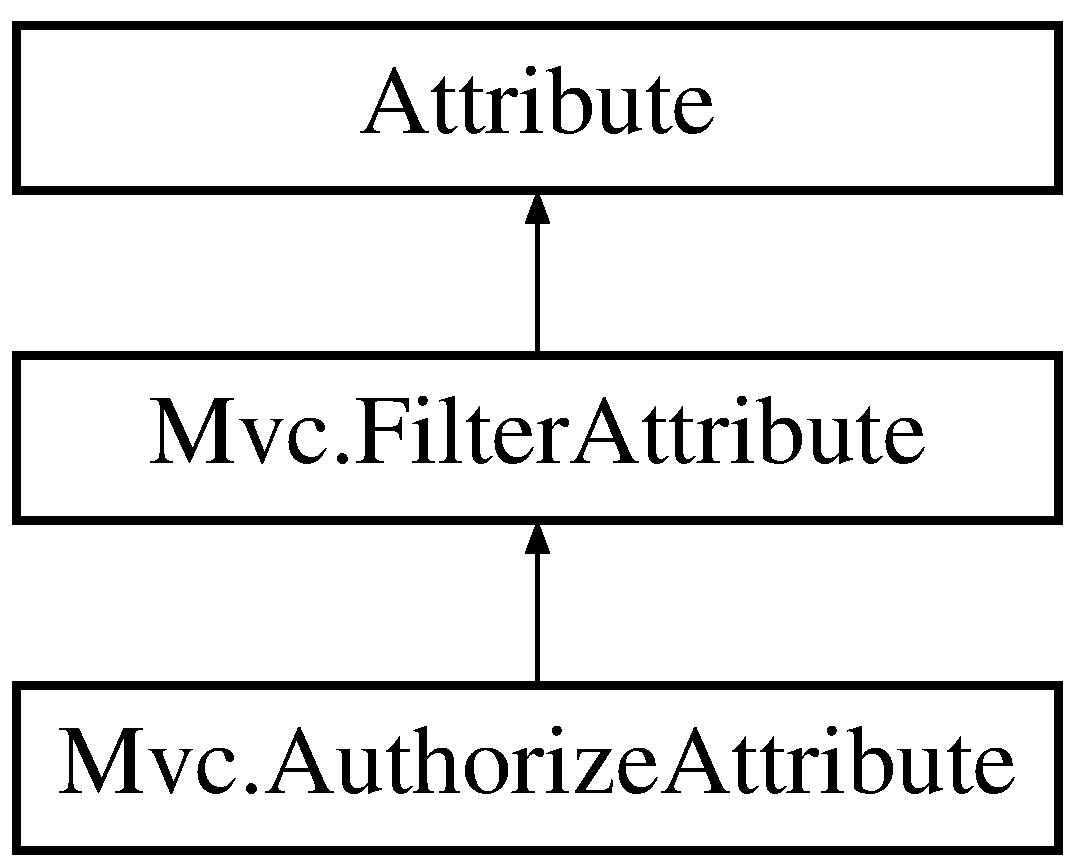
\includegraphics[height=3.000000cm]{class_mvc_1_1_authorize_attribute}
\end{center}
\end{figure}
\subsection*{Public Member Functions}
\begin{DoxyCompactItemize}
\item 
\hyperlink{class_mvc_1_1_user}{User} \hyperlink{class_mvc_1_1_authorize_attribute_a6e307e8177daede23e820c499990cf69}{Authorize\+Auth\+Token} (\hyperlink{class_mvc_1_1_request}{Request} request, string secret)
\begin{DoxyCompactList}\small\item\em Authorize an incoming Auth Token and returns the corresponded user or null if is not valid. \end{DoxyCompactList}\item 
\hyperlink{class_mvc_1_1_user}{User} \hyperlink{class_mvc_1_1_authorize_attribute_aad3c74835450cca65e86f79aca028de4}{Authorize\+Session} (string session)
\begin{DoxyCompactList}\small\item\em Authorize session and returns the corresponded user or null if is not valid. \end{DoxyCompactList}\end{DoxyCompactItemize}


\subsection{Detailed Description}
Representative class of an authorization attribute for the controllers methods. 



Definition at line 17 of file Authorize\+Attribute.\+cs.



\subsection{Member Function Documentation}
\mbox{\Hypertarget{class_mvc_1_1_authorize_attribute_a6e307e8177daede23e820c499990cf69}\label{class_mvc_1_1_authorize_attribute_a6e307e8177daede23e820c499990cf69}} 
\index{Mvc\+::\+Authorize\+Attribute@{Mvc\+::\+Authorize\+Attribute}!Authorize\+Auth\+Token@{Authorize\+Auth\+Token}}
\index{Authorize\+Auth\+Token@{Authorize\+Auth\+Token}!Mvc\+::\+Authorize\+Attribute@{Mvc\+::\+Authorize\+Attribute}}
\subsubsection{\texorpdfstring{Authorize\+Auth\+Token()}{AuthorizeAuthToken()}}
{\footnotesize\ttfamily \hyperlink{class_mvc_1_1_user}{User} Mvc.\+Authorize\+Attribute.\+Authorize\+Auth\+Token (\begin{DoxyParamCaption}\item[{\hyperlink{class_mvc_1_1_request}{Request}}]{request,  }\item[{string}]{secret }\end{DoxyParamCaption})}



Authorize an incoming Auth Token and returns the corresponded user or null if is not valid. 


\begin{DoxyParams}{Parameters}
{\em request} & A \hyperlink{class_mvc_1_1_request}{Request} instance with the incoming request information.\\
\hline
{\em secret} & A string representing the secret key to encode and decode the token.\\
\hline
\end{DoxyParams}
\begin{DoxyReturn}{Returns}
Corresponded \hyperlink{class_mvc_1_1_user}{User} of the token, or null if is not valid
\end{DoxyReturn}


Definition at line 25 of file Authorize\+Attribute.\+cs.

\mbox{\Hypertarget{class_mvc_1_1_authorize_attribute_aad3c74835450cca65e86f79aca028de4}\label{class_mvc_1_1_authorize_attribute_aad3c74835450cca65e86f79aca028de4}} 
\index{Mvc\+::\+Authorize\+Attribute@{Mvc\+::\+Authorize\+Attribute}!Authorize\+Session@{Authorize\+Session}}
\index{Authorize\+Session@{Authorize\+Session}!Mvc\+::\+Authorize\+Attribute@{Mvc\+::\+Authorize\+Attribute}}
\subsubsection{\texorpdfstring{Authorize\+Session()}{AuthorizeSession()}}
{\footnotesize\ttfamily \hyperlink{class_mvc_1_1_user}{User} Mvc.\+Authorize\+Attribute.\+Authorize\+Session (\begin{DoxyParamCaption}\item[{string}]{session }\end{DoxyParamCaption})}



Authorize session and returns the corresponded user or null if is not valid. 


\begin{DoxyParams}{Parameters}
{\em session} & A string the presenting the session\\
\hline
\end{DoxyParams}
\begin{DoxyReturn}{Returns}
Corresponded \hyperlink{class_mvc_1_1_user}{User} of the token, or null if is not valid
\end{DoxyReturn}


Definition at line 60 of file Authorize\+Attribute.\+cs.



The documentation for this class was generated from the following file\+:\begin{DoxyCompactItemize}
\item 
C\+:/\+Users/dieguito12/\+Code/sharpener-\/framework/src/\+Mvc/Authorize\+Attribute.\+cs\end{DoxyCompactItemize}

\hypertarget{class_mvc_1_1_base_controller}{}\section{Mvc.\+Base\+Controller Class Reference}
\label{class_mvc_1_1_base_controller}\index{Mvc.\+Base\+Controller@{Mvc.\+Base\+Controller}}


Representative class of a base controller  


\subsection*{Public Member Functions}
\begin{DoxyCompactItemize}
\item 
void \hyperlink{class_mvc_1_1_base_controller_ae29f489a7f1a4829301aac4c4f762d1d}{Unset\+User} ()
\begin{DoxyCompactList}\small\item\em Unsets the current user. \end{DoxyCompactList}\item 
\hyperlink{class_mvc_1_1_base_controller_a5d30ca8bf9e277187b8212fb6b8a8428}{Base\+Controller} ()
\begin{DoxyCompactList}\small\item\em Constructor of the \hyperlink{class_mvc_1_1_base_controller}{Base\+Controller} class. \end{DoxyCompactList}\item 
\hyperlink{interface_mvc_1_1_i_action_result}{I\+Action\+Result} \hyperlink{class_mvc_1_1_base_controller_ac13791a92c035d9c60d7193676e88c2c}{Json} (string json, int code)
\begin{DoxyCompactList}\small\item\em Creates a new \hyperlink{class_mvc_1_1_json}{Json} response \end{DoxyCompactList}\item 
\hyperlink{interface_mvc_1_1_i_action_result}{I\+Action\+Result} \hyperlink{class_mvc_1_1_base_controller_a391c25d6786a328c92aa81a786786a21}{Content} (string text, int code, string redirect)
\begin{DoxyCompactList}\small\item\em Creates a new \hyperlink{class_mvc_1_1_content}{Content} response \end{DoxyCompactList}\item 
\hyperlink{interface_mvc_1_1_i_action_result}{I\+Action\+Result} \hyperlink{class_mvc_1_1_base_controller_a572c7ba4224b5596962be6cd6311fe50}{View} (string template, object data, int code)
\begin{DoxyCompactList}\small\item\em Creates a new \hyperlink{class_mvc_1_1_view}{View} response \end{DoxyCompactList}\end{DoxyCompactItemize}
\subsection*{Properties}
\begin{DoxyCompactItemize}
\item 
\hyperlink{class_mvc_1_1_http_context}{Http\+Context} \hyperlink{class_mvc_1_1_base_controller_ad7b4a9abd6951cae8d4220a4ccea783d}{Http\+Context}\hspace{0.3cm}{\ttfamily  \mbox{[}get, set\mbox{]}}
\begin{DoxyCompactList}\small\item\em A context information from the http server. \end{DoxyCompactList}\item 
\hyperlink{class_mvc_1_1_request}{Request} \hyperlink{class_mvc_1_1_base_controller_a72a2384832ba902229f295157ad71282}{Http\+Request}\hspace{0.3cm}{\ttfamily  \mbox{[}get, set\mbox{]}}
\begin{DoxyCompactList}\small\item\em The incoming request from the server. \end{DoxyCompactList}\item 
\hyperlink{class_mvc_1_1_route}{Route} \hyperlink{class_mvc_1_1_base_controller_a860c6d8a5ffdadec5f46d2baeaa20186}{Route}\hspace{0.3cm}{\ttfamily  \mbox{[}get, set\mbox{]}}
\begin{DoxyCompactList}\small\item\em The current route that is being used. \end{DoxyCompactList}\item 
Dictionary$<$ string, object $>$ \hyperlink{class_mvc_1_1_base_controller_ac9ec764bde3833c4da076a64b0f3d0cc}{Session}\hspace{0.3cm}{\ttfamily  \mbox{[}get, set\mbox{]}}
\begin{DoxyCompactList}\small\item\em A session dictionary to store volatile data. \end{DoxyCompactList}\item 
\hyperlink{class_mvc_1_1_user}{User} \hyperlink{class_mvc_1_1_base_controller_a441230929ad77f983c662d419474c41a}{User}\hspace{0.3cm}{\ttfamily  \mbox{[}get, set\mbox{]}}
\begin{DoxyCompactList}\small\item\em Gets of sets the current user \end{DoxyCompactList}\end{DoxyCompactItemize}


\subsection{Detailed Description}
Representative class of a base controller 



Definition at line 16 of file Base\+Controller.\+cs.



\subsection{Constructor \& Destructor Documentation}
\mbox{\Hypertarget{class_mvc_1_1_base_controller_a5d30ca8bf9e277187b8212fb6b8a8428}\label{class_mvc_1_1_base_controller_a5d30ca8bf9e277187b8212fb6b8a8428}} 
\index{Mvc\+::\+Base\+Controller@{Mvc\+::\+Base\+Controller}!Base\+Controller@{Base\+Controller}}
\index{Base\+Controller@{Base\+Controller}!Mvc\+::\+Base\+Controller@{Mvc\+::\+Base\+Controller}}
\subsubsection{\texorpdfstring{Base\+Controller()}{BaseController()}}
{\footnotesize\ttfamily Mvc.\+Base\+Controller.\+Base\+Controller (\begin{DoxyParamCaption}{ }\end{DoxyParamCaption})}



Constructor of the \hyperlink{class_mvc_1_1_base_controller}{Base\+Controller} class. 



Definition at line 124 of file Base\+Controller.\+cs.



\subsection{Member Function Documentation}
\mbox{\Hypertarget{class_mvc_1_1_base_controller_a391c25d6786a328c92aa81a786786a21}\label{class_mvc_1_1_base_controller_a391c25d6786a328c92aa81a786786a21}} 
\index{Mvc\+::\+Base\+Controller@{Mvc\+::\+Base\+Controller}!Content@{Content}}
\index{Content@{Content}!Mvc\+::\+Base\+Controller@{Mvc\+::\+Base\+Controller}}
\subsubsection{\texorpdfstring{Content()}{Content()}}
{\footnotesize\ttfamily \hyperlink{interface_mvc_1_1_i_action_result}{I\+Action\+Result} Mvc.\+Base\+Controller.\+Content (\begin{DoxyParamCaption}\item[{string}]{text,  }\item[{int}]{code,  }\item[{string}]{redirect }\end{DoxyParamCaption})}



Creates a new \hyperlink{class_mvc_1_1_content}{Content} response 


\begin{DoxyParams}{Parameters}
{\em text} & A string of raw text of the response\\
\hline
{\em code} & An int representing the status code\\
\hline
{\em redirect} & A string representing the redirection url\\
\hline
\end{DoxyParams}
\begin{DoxyReturn}{Returns}
A \hyperlink{class_mvc_1_1_content}{Content} object with the response
\end{DoxyReturn}


Definition at line 157 of file Base\+Controller.\+cs.

\mbox{\Hypertarget{class_mvc_1_1_base_controller_ac13791a92c035d9c60d7193676e88c2c}\label{class_mvc_1_1_base_controller_ac13791a92c035d9c60d7193676e88c2c}} 
\index{Mvc\+::\+Base\+Controller@{Mvc\+::\+Base\+Controller}!Json@{Json}}
\index{Json@{Json}!Mvc\+::\+Base\+Controller@{Mvc\+::\+Base\+Controller}}
\subsubsection{\texorpdfstring{Json()}{Json()}}
{\footnotesize\ttfamily \hyperlink{interface_mvc_1_1_i_action_result}{I\+Action\+Result} Mvc.\+Base\+Controller.\+Json (\begin{DoxyParamCaption}\item[{string}]{json,  }\item[{int}]{code }\end{DoxyParamCaption})}



Creates a new \hyperlink{class_mvc_1_1_json}{Json} response 


\begin{DoxyParams}{Parameters}
{\em json} & A string representing the json to respond.\\
\hline
{\em code} & An int representing the status code.\\
\hline
\end{DoxyParams}
\begin{DoxyReturn}{Returns}
A \hyperlink{class_mvc_1_1_json}{Json} object with the response.
\end{DoxyReturn}


Definition at line 145 of file Base\+Controller.\+cs.

\mbox{\Hypertarget{class_mvc_1_1_base_controller_ae29f489a7f1a4829301aac4c4f762d1d}\label{class_mvc_1_1_base_controller_ae29f489a7f1a4829301aac4c4f762d1d}} 
\index{Mvc\+::\+Base\+Controller@{Mvc\+::\+Base\+Controller}!Unset\+User@{Unset\+User}}
\index{Unset\+User@{Unset\+User}!Mvc\+::\+Base\+Controller@{Mvc\+::\+Base\+Controller}}
\subsubsection{\texorpdfstring{Unset\+User()}{UnsetUser()}}
{\footnotesize\ttfamily void Mvc.\+Base\+Controller.\+Unset\+User (\begin{DoxyParamCaption}{ }\end{DoxyParamCaption})}



Unsets the current user. 



Definition at line 100 of file Base\+Controller.\+cs.

\mbox{\Hypertarget{class_mvc_1_1_base_controller_a572c7ba4224b5596962be6cd6311fe50}\label{class_mvc_1_1_base_controller_a572c7ba4224b5596962be6cd6311fe50}} 
\index{Mvc\+::\+Base\+Controller@{Mvc\+::\+Base\+Controller}!View@{View}}
\index{View@{View}!Mvc\+::\+Base\+Controller@{Mvc\+::\+Base\+Controller}}
\subsubsection{\texorpdfstring{View()}{View()}}
{\footnotesize\ttfamily \hyperlink{interface_mvc_1_1_i_action_result}{I\+Action\+Result} Mvc.\+Base\+Controller.\+View (\begin{DoxyParamCaption}\item[{string}]{template,  }\item[{object}]{data,  }\item[{int}]{code }\end{DoxyParamCaption})}



Creates a new \hyperlink{class_mvc_1_1_view}{View} response 


\begin{DoxyParams}{Parameters}
{\em template} & A string representing the name of the view template.\\
\hline
{\em data} & An object with the data to be passed to the view template.\\
\hline
{\em code} & An int representing the status code.\\
\hline
\end{DoxyParams}
\begin{DoxyReturn}{Returns}
A \hyperlink{class_mvc_1_1_view}{View} object with the response data.
\end{DoxyReturn}


Definition at line 169 of file Base\+Controller.\+cs.



\subsection{Property Documentation}
\mbox{\Hypertarget{class_mvc_1_1_base_controller_ad7b4a9abd6951cae8d4220a4ccea783d}\label{class_mvc_1_1_base_controller_ad7b4a9abd6951cae8d4220a4ccea783d}} 
\index{Mvc\+::\+Base\+Controller@{Mvc\+::\+Base\+Controller}!Http\+Context@{Http\+Context}}
\index{Http\+Context@{Http\+Context}!Mvc\+::\+Base\+Controller@{Mvc\+::\+Base\+Controller}}
\subsubsection{\texorpdfstring{Http\+Context}{HttpContext}}
{\footnotesize\ttfamily \hyperlink{class_mvc_1_1_http_context}{Http\+Context} Mvc.\+Base\+Controller.\+Http\+Context\hspace{0.3cm}{\ttfamily [get]}, {\ttfamily [set]}}



A context information from the http server. 



Definition at line 27 of file Base\+Controller.\+cs.

\mbox{\Hypertarget{class_mvc_1_1_base_controller_a72a2384832ba902229f295157ad71282}\label{class_mvc_1_1_base_controller_a72a2384832ba902229f295157ad71282}} 
\index{Mvc\+::\+Base\+Controller@{Mvc\+::\+Base\+Controller}!Http\+Request@{Http\+Request}}
\index{Http\+Request@{Http\+Request}!Mvc\+::\+Base\+Controller@{Mvc\+::\+Base\+Controller}}
\subsubsection{\texorpdfstring{Http\+Request}{HttpRequest}}
{\footnotesize\ttfamily \hyperlink{class_mvc_1_1_request}{Request} Mvc.\+Base\+Controller.\+Http\+Request\hspace{0.3cm}{\ttfamily [get]}, {\ttfamily [set]}}



The incoming request from the server. 



Definition at line 36 of file Base\+Controller.\+cs.

\mbox{\Hypertarget{class_mvc_1_1_base_controller_a860c6d8a5ffdadec5f46d2baeaa20186}\label{class_mvc_1_1_base_controller_a860c6d8a5ffdadec5f46d2baeaa20186}} 
\index{Mvc\+::\+Base\+Controller@{Mvc\+::\+Base\+Controller}!Route@{Route}}
\index{Route@{Route}!Mvc\+::\+Base\+Controller@{Mvc\+::\+Base\+Controller}}
\subsubsection{\texorpdfstring{Route}{Route}}
{\footnotesize\ttfamily \hyperlink{class_mvc_1_1_route}{Route} Mvc.\+Base\+Controller.\+Route\hspace{0.3cm}{\ttfamily [get]}, {\ttfamily [set]}}



The current route that is being used. 



Definition at line 45 of file Base\+Controller.\+cs.

\mbox{\Hypertarget{class_mvc_1_1_base_controller_ac9ec764bde3833c4da076a64b0f3d0cc}\label{class_mvc_1_1_base_controller_ac9ec764bde3833c4da076a64b0f3d0cc}} 
\index{Mvc\+::\+Base\+Controller@{Mvc\+::\+Base\+Controller}!Session@{Session}}
\index{Session@{Session}!Mvc\+::\+Base\+Controller@{Mvc\+::\+Base\+Controller}}
\subsubsection{\texorpdfstring{Session}{Session}}
{\footnotesize\ttfamily Dictionary$<$string, object$>$ Mvc.\+Base\+Controller.\+Session\hspace{0.3cm}{\ttfamily [get]}, {\ttfamily [set]}}



A session dictionary to store volatile data. 



Definition at line 54 of file Base\+Controller.\+cs.

\mbox{\Hypertarget{class_mvc_1_1_base_controller_a441230929ad77f983c662d419474c41a}\label{class_mvc_1_1_base_controller_a441230929ad77f983c662d419474c41a}} 
\index{Mvc\+::\+Base\+Controller@{Mvc\+::\+Base\+Controller}!User@{User}}
\index{User@{User}!Mvc\+::\+Base\+Controller@{Mvc\+::\+Base\+Controller}}
\subsubsection{\texorpdfstring{User}{User}}
{\footnotesize\ttfamily \hyperlink{class_mvc_1_1_user}{User} Mvc.\+Base\+Controller.\+User\hspace{0.3cm}{\ttfamily [get]}, {\ttfamily [set]}}



Gets of sets the current user 

When it is set it is validated if is using the jwt driver

Definition at line 64 of file Base\+Controller.\+cs.



The documentation for this class was generated from the following file\+:\begin{DoxyCompactItemize}
\item 
C\+:/\+Users/dieguito12/\+Code/sharpener-\/framework/src/\+Mvc/Base\+Controller.\+cs\end{DoxyCompactItemize}

\hypertarget{class_mvc_1_1_configuration_manager}{}\section{Mvc.\+Configuration\+Manager Class Reference}
\label{class_mvc_1_1_configuration_manager}\index{Mvc.\+Configuration\+Manager@{Mvc.\+Configuration\+Manager}}


Representative class of an app configuration manager.  


\subsection*{Public Member Functions}
\begin{DoxyCompactItemize}
\item 
\hyperlink{class_mvc_1_1_configuration_manager_aa7a6bcdf5a3f46717d269896a2d822b1}{Configuration\+Manager} (string app\+Config\+Path)
\begin{DoxyCompactList}\small\item\em Constructor of the \hyperlink{class_mvc_1_1_configuration_manager}{Configuration\+Manager} class \end{DoxyCompactList}\end{DoxyCompactItemize}
\subsection*{Properties}
\begin{DoxyCompactItemize}
\item 
string \hyperlink{class_mvc_1_1_configuration_manager_a29c7dc729909b9ad5e1a9e8ede9a3884}{Application\+Name}\hspace{0.3cm}{\ttfamily  \mbox{[}get\mbox{]}}
\begin{DoxyCompactList}\small\item\em Gets the application name. \end{DoxyCompactList}\item 
string \hyperlink{class_mvc_1_1_configuration_manager_a208b34447455d80d11bfe95905b90c7c}{Application\+Secret\+Key}\hspace{0.3cm}{\ttfamily  \mbox{[}get\mbox{]}}
\begin{DoxyCompactList}\small\item\em Gets the application secret key. \end{DoxyCompactList}\item 
Dictionary$<$ int, string $>$ \hyperlink{class_mvc_1_1_configuration_manager_aae59944b7a43dba20df4658860c5c1c4}{Application\+Error\+Pages}\hspace{0.3cm}{\ttfamily  \mbox{[}get\mbox{]}}
\begin{DoxyCompactList}\small\item\em Gets the error pages dictionary. \end{DoxyCompactList}\item 
string \hyperlink{class_mvc_1_1_configuration_manager_a0cb7f0a9c20b0f5f67e9bdac41496172}{Application\+Authentication\+Driver}\hspace{0.3cm}{\ttfamily  \mbox{[}get\mbox{]}}
\begin{DoxyCompactList}\small\item\em Gets the application authentication driver. \end{DoxyCompactList}\item 
string \hyperlink{class_mvc_1_1_configuration_manager_a318a7ee1d3119f9bc651adfbd512e627}{Application\+Database\+Connection}\hspace{0.3cm}{\ttfamily  \mbox{[}get\mbox{]}}
\begin{DoxyCompactList}\small\item\em Gets the application database connection string. \end{DoxyCompactList}\item 
string \hyperlink{class_mvc_1_1_configuration_manager_a2384d0345e8093089dfff959c07e562e}{Applicaiton\+Default\+Document}\hspace{0.3cm}{\ttfamily  \mbox{[}get\mbox{]}}
\begin{DoxyCompactList}\small\item\em Gets the application default document name. \end{DoxyCompactList}\end{DoxyCompactItemize}


\subsection{Detailed Description}
Representative class of an app configuration manager. 



Definition at line 14 of file Configuration\+Manager .\+cs.



\subsection{Constructor \& Destructor Documentation}
\mbox{\Hypertarget{class_mvc_1_1_configuration_manager_aa7a6bcdf5a3f46717d269896a2d822b1}\label{class_mvc_1_1_configuration_manager_aa7a6bcdf5a3f46717d269896a2d822b1}} 
\index{Mvc\+::\+Configuration\+Manager@{Mvc\+::\+Configuration\+Manager}!Configuration\+Manager@{Configuration\+Manager}}
\index{Configuration\+Manager@{Configuration\+Manager}!Mvc\+::\+Configuration\+Manager@{Mvc\+::\+Configuration\+Manager}}
\subsubsection{\texorpdfstring{Configuration\+Manager()}{ConfigurationManager()}}
{\footnotesize\ttfamily Mvc.\+Configuration\+Manager.\+Configuration\+Manager (\begin{DoxyParamCaption}\item[{string}]{app\+Config\+Path }\end{DoxyParamCaption})}



Constructor of the \hyperlink{class_mvc_1_1_configuration_manager}{Configuration\+Manager} class 


\begin{DoxyParams}{Parameters}
{\em app\+Config\+Path} & A string representing the path of the configuration file\\
\hline
\end{DoxyParams}


Definition at line 20 of file Configuration\+Manager .\+cs.



\subsection{Property Documentation}
\mbox{\Hypertarget{class_mvc_1_1_configuration_manager_a2384d0345e8093089dfff959c07e562e}\label{class_mvc_1_1_configuration_manager_a2384d0345e8093089dfff959c07e562e}} 
\index{Mvc\+::\+Configuration\+Manager@{Mvc\+::\+Configuration\+Manager}!Applicaiton\+Default\+Document@{Applicaiton\+Default\+Document}}
\index{Applicaiton\+Default\+Document@{Applicaiton\+Default\+Document}!Mvc\+::\+Configuration\+Manager@{Mvc\+::\+Configuration\+Manager}}
\subsubsection{\texorpdfstring{Applicaiton\+Default\+Document}{ApplicaitonDefaultDocument}}
{\footnotesize\ttfamily string Mvc.\+Configuration\+Manager.\+Applicaiton\+Default\+Document\hspace{0.3cm}{\ttfamily [get]}}



Gets the application default document name. 



Definition at line 98 of file Configuration\+Manager .\+cs.

\mbox{\Hypertarget{class_mvc_1_1_configuration_manager_a0cb7f0a9c20b0f5f67e9bdac41496172}\label{class_mvc_1_1_configuration_manager_a0cb7f0a9c20b0f5f67e9bdac41496172}} 
\index{Mvc\+::\+Configuration\+Manager@{Mvc\+::\+Configuration\+Manager}!Application\+Authentication\+Driver@{Application\+Authentication\+Driver}}
\index{Application\+Authentication\+Driver@{Application\+Authentication\+Driver}!Mvc\+::\+Configuration\+Manager@{Mvc\+::\+Configuration\+Manager}}
\subsubsection{\texorpdfstring{Application\+Authentication\+Driver}{ApplicationAuthenticationDriver}}
{\footnotesize\ttfamily string Mvc.\+Configuration\+Manager.\+Application\+Authentication\+Driver\hspace{0.3cm}{\ttfamily [get]}}



Gets the application authentication driver. 



Definition at line 80 of file Configuration\+Manager .\+cs.

\mbox{\Hypertarget{class_mvc_1_1_configuration_manager_a318a7ee1d3119f9bc651adfbd512e627}\label{class_mvc_1_1_configuration_manager_a318a7ee1d3119f9bc651adfbd512e627}} 
\index{Mvc\+::\+Configuration\+Manager@{Mvc\+::\+Configuration\+Manager}!Application\+Database\+Connection@{Application\+Database\+Connection}}
\index{Application\+Database\+Connection@{Application\+Database\+Connection}!Mvc\+::\+Configuration\+Manager@{Mvc\+::\+Configuration\+Manager}}
\subsubsection{\texorpdfstring{Application\+Database\+Connection}{ApplicationDatabaseConnection}}
{\footnotesize\ttfamily string Mvc.\+Configuration\+Manager.\+Application\+Database\+Connection\hspace{0.3cm}{\ttfamily [get]}}



Gets the application database connection string. 



Definition at line 89 of file Configuration\+Manager .\+cs.

\mbox{\Hypertarget{class_mvc_1_1_configuration_manager_aae59944b7a43dba20df4658860c5c1c4}\label{class_mvc_1_1_configuration_manager_aae59944b7a43dba20df4658860c5c1c4}} 
\index{Mvc\+::\+Configuration\+Manager@{Mvc\+::\+Configuration\+Manager}!Application\+Error\+Pages@{Application\+Error\+Pages}}
\index{Application\+Error\+Pages@{Application\+Error\+Pages}!Mvc\+::\+Configuration\+Manager@{Mvc\+::\+Configuration\+Manager}}
\subsubsection{\texorpdfstring{Application\+Error\+Pages}{ApplicationErrorPages}}
{\footnotesize\ttfamily Dictionary$<$int, string$>$ Mvc.\+Configuration\+Manager.\+Application\+Error\+Pages\hspace{0.3cm}{\ttfamily [get]}}



Gets the error pages dictionary. 



Definition at line 71 of file Configuration\+Manager .\+cs.

\mbox{\Hypertarget{class_mvc_1_1_configuration_manager_a29c7dc729909b9ad5e1a9e8ede9a3884}\label{class_mvc_1_1_configuration_manager_a29c7dc729909b9ad5e1a9e8ede9a3884}} 
\index{Mvc\+::\+Configuration\+Manager@{Mvc\+::\+Configuration\+Manager}!Application\+Name@{Application\+Name}}
\index{Application\+Name@{Application\+Name}!Mvc\+::\+Configuration\+Manager@{Mvc\+::\+Configuration\+Manager}}
\subsubsection{\texorpdfstring{Application\+Name}{ApplicationName}}
{\footnotesize\ttfamily string Mvc.\+Configuration\+Manager.\+Application\+Name\hspace{0.3cm}{\ttfamily [get]}}



Gets the application name. 



Definition at line 53 of file Configuration\+Manager .\+cs.

\mbox{\Hypertarget{class_mvc_1_1_configuration_manager_a208b34447455d80d11bfe95905b90c7c}\label{class_mvc_1_1_configuration_manager_a208b34447455d80d11bfe95905b90c7c}} 
\index{Mvc\+::\+Configuration\+Manager@{Mvc\+::\+Configuration\+Manager}!Application\+Secret\+Key@{Application\+Secret\+Key}}
\index{Application\+Secret\+Key@{Application\+Secret\+Key}!Mvc\+::\+Configuration\+Manager@{Mvc\+::\+Configuration\+Manager}}
\subsubsection{\texorpdfstring{Application\+Secret\+Key}{ApplicationSecretKey}}
{\footnotesize\ttfamily string Mvc.\+Configuration\+Manager.\+Application\+Secret\+Key\hspace{0.3cm}{\ttfamily [get]}}



Gets the application secret key. 



Definition at line 62 of file Configuration\+Manager .\+cs.



The documentation for this class was generated from the following file\+:\begin{DoxyCompactItemize}
\item 
C\+:/\+Users/dieguito12/\+Code/sharpener-\/framework/src/\+Mvc/Configuration\+Manager .\+cs\end{DoxyCompactItemize}

\hypertarget{class_mvc_1_1_content}{}\section{Mvc.\+Content Class Reference}
\label{class_mvc_1_1_content}\index{Mvc.\+Content@{Mvc.\+Content}}


Representative class of a raw content (or redirection) response of a controller  


Inheritance diagram for Mvc.\+Content\+:\begin{figure}[H]
\begin{center}
\leavevmode
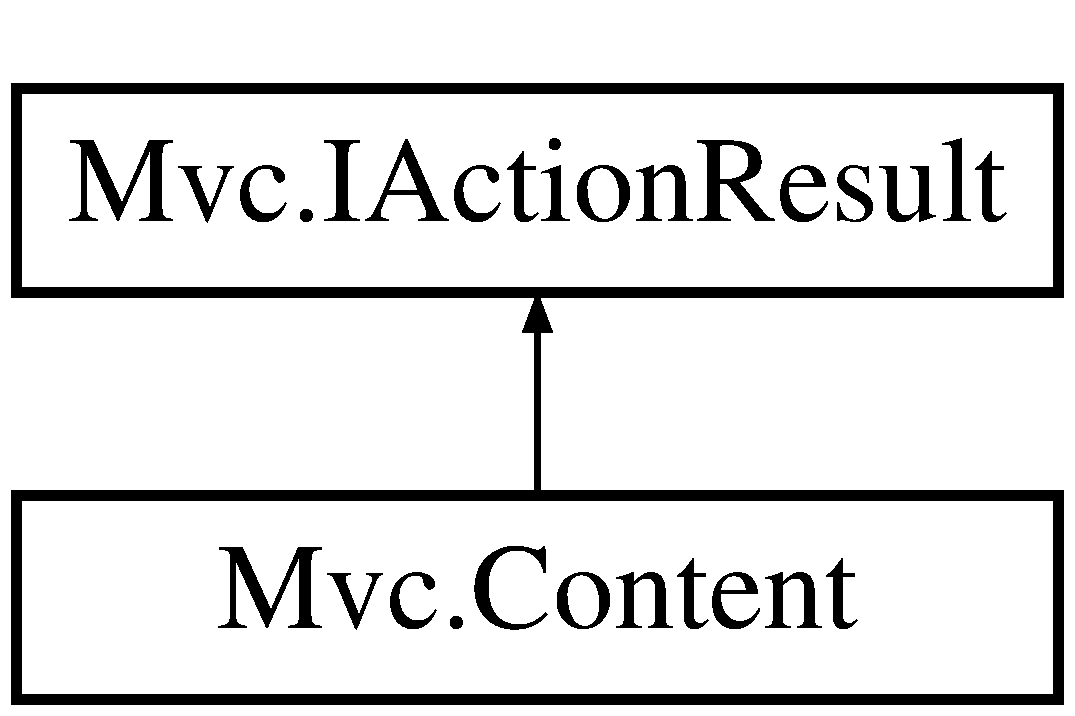
\includegraphics[height=2.000000cm]{class_mvc_1_1_content}
\end{center}
\end{figure}
\subsection*{Public Member Functions}
\begin{DoxyCompactItemize}
\item 
\hyperlink{class_mvc_1_1_content_aabb482c66606b1eff2ac79ce3558c175}{Content} (string text, int code, string redirect)
\begin{DoxyCompactList}\small\item\em Constructor of the \hyperlink{class_mvc_1_1_content}{Content} class \end{DoxyCompactList}\item 
int \hyperlink{class_mvc_1_1_content_a77175a25c002834c59e14cde60719c28}{Code} ()
\begin{DoxyCompactList}\small\item\em Gets the status code of the response. \end{DoxyCompactList}\item 
Memory\+Stream \hyperlink{class_mvc_1_1_content_aabe147bc684eed8af000906fbfe92b61}{Response} ()
\begin{DoxyCompactList}\small\item\em Gets the response of the controller in a stream. \end{DoxyCompactList}\item 
string \hyperlink{class_mvc_1_1_content_a5d384ef7d466dfc88ccf1eb7f10728ad}{Content\+Type} ()
\begin{DoxyCompactList}\small\item\em Gets the content type of the response. \end{DoxyCompactList}\item 
string \hyperlink{class_mvc_1_1_content_ae4eba27dbea637dc61bc4b681f731545}{Redirection} ()
\begin{DoxyCompactList}\small\item\em Gets the url where the response is going to redirect (if there is any). \end{DoxyCompactList}\end{DoxyCompactItemize}


\subsection{Detailed Description}
Representative class of a raw content (or redirection) response of a controller 



Definition at line 13 of file Content.\+cs.



\subsection{Constructor \& Destructor Documentation}
\mbox{\Hypertarget{class_mvc_1_1_content_aabb482c66606b1eff2ac79ce3558c175}\label{class_mvc_1_1_content_aabb482c66606b1eff2ac79ce3558c175}} 
\index{Mvc\+::\+Content@{Mvc\+::\+Content}!Content@{Content}}
\index{Content@{Content}!Mvc\+::\+Content@{Mvc\+::\+Content}}
\subsubsection{\texorpdfstring{Content()}{Content()}}
{\footnotesize\ttfamily Mvc.\+Content.\+Content (\begin{DoxyParamCaption}\item[{string}]{text,  }\item[{int}]{code,  }\item[{string}]{redirect }\end{DoxyParamCaption})}



Constructor of the \hyperlink{class_mvc_1_1_content}{Content} class 


\begin{DoxyParams}{Parameters}
{\em text} & A string of raw text of the response\\
\hline
{\em code} & An int representing the status code\\
\hline
{\em redirect} & A string representing the redirection url\\
\hline
\end{DoxyParams}


Definition at line 36 of file Content.\+cs.



\subsection{Member Function Documentation}
\mbox{\Hypertarget{class_mvc_1_1_content_a77175a25c002834c59e14cde60719c28}\label{class_mvc_1_1_content_a77175a25c002834c59e14cde60719c28}} 
\index{Mvc\+::\+Content@{Mvc\+::\+Content}!Code@{Code}}
\index{Code@{Code}!Mvc\+::\+Content@{Mvc\+::\+Content}}
\subsubsection{\texorpdfstring{Code()}{Code()}}
{\footnotesize\ttfamily int Mvc.\+Content.\+Code (\begin{DoxyParamCaption}{ }\end{DoxyParamCaption})}



Gets the status code of the response. 

\begin{DoxyReturn}{Returns}
An int representing the status code
\end{DoxyReturn}


Implements \hyperlink{interface_mvc_1_1_i_action_result_ab6b85ae50597587395df99b972c3d26b}{Mvc.\+I\+Action\+Result}.



Definition at line 47 of file Content.\+cs.

\mbox{\Hypertarget{class_mvc_1_1_content_a5d384ef7d466dfc88ccf1eb7f10728ad}\label{class_mvc_1_1_content_a5d384ef7d466dfc88ccf1eb7f10728ad}} 
\index{Mvc\+::\+Content@{Mvc\+::\+Content}!Content\+Type@{Content\+Type}}
\index{Content\+Type@{Content\+Type}!Mvc\+::\+Content@{Mvc\+::\+Content}}
\subsubsection{\texorpdfstring{Content\+Type()}{ContentType()}}
{\footnotesize\ttfamily string Mvc.\+Content.\+Content\+Type (\begin{DoxyParamCaption}{ }\end{DoxyParamCaption})}



Gets the content type of the response. 

\begin{DoxyReturn}{Returns}
A string representing the content type of the response
\end{DoxyReturn}


Implements \hyperlink{interface_mvc_1_1_i_action_result_a8ad08f29bba90dfbe06d7a00465af10a}{Mvc.\+I\+Action\+Result}.



Definition at line 70 of file Content.\+cs.

\mbox{\Hypertarget{class_mvc_1_1_content_ae4eba27dbea637dc61bc4b681f731545}\label{class_mvc_1_1_content_ae4eba27dbea637dc61bc4b681f731545}} 
\index{Mvc\+::\+Content@{Mvc\+::\+Content}!Redirection@{Redirection}}
\index{Redirection@{Redirection}!Mvc\+::\+Content@{Mvc\+::\+Content}}
\subsubsection{\texorpdfstring{Redirection()}{Redirection()}}
{\footnotesize\ttfamily string Mvc.\+Content.\+Redirection (\begin{DoxyParamCaption}{ }\end{DoxyParamCaption})}



Gets the url where the response is going to redirect (if there is any). 

\begin{DoxyReturn}{Returns}
A string representing the redirection url
\end{DoxyReturn}


Implements \hyperlink{interface_mvc_1_1_i_action_result_a036707da116ea300eae90e105b8d1ced}{Mvc.\+I\+Action\+Result}.



Definition at line 79 of file Content.\+cs.

\mbox{\Hypertarget{class_mvc_1_1_content_aabe147bc684eed8af000906fbfe92b61}\label{class_mvc_1_1_content_aabe147bc684eed8af000906fbfe92b61}} 
\index{Mvc\+::\+Content@{Mvc\+::\+Content}!Response@{Response}}
\index{Response@{Response}!Mvc\+::\+Content@{Mvc\+::\+Content}}
\subsubsection{\texorpdfstring{Response()}{Response()}}
{\footnotesize\ttfamily Memory\+Stream Mvc.\+Content.\+Response (\begin{DoxyParamCaption}{ }\end{DoxyParamCaption})}



Gets the response of the controller in a stream. 

\begin{DoxyReturn}{Returns}
Memory\+Stream that represents the response of the controller.
\end{DoxyReturn}


Implements \hyperlink{interface_mvc_1_1_i_action_result_a7cf7423071384c7b2bac75a5f4d6e25c}{Mvc.\+I\+Action\+Result}.



Definition at line 56 of file Content.\+cs.



The documentation for this class was generated from the following file\+:\begin{DoxyCompactItemize}
\item 
C\+:/\+Users/dieguito12/\+Code/sharpener-\/framework/src/\+Mvc/Content.\+cs\end{DoxyCompactItemize}

\hypertarget{class_mvc_1_1_filter_attribute}{}\section{Mvc.\+Filter\+Attribute Class Reference}
\label{class_mvc_1_1_filter_attribute}\index{Mvc.\+Filter\+Attribute@{Mvc.\+Filter\+Attribute}}


Representative abstract class of a filter attribute.  


Inheritance diagram for Mvc.\+Filter\+Attribute\+:\begin{figure}[H]
\begin{center}
\leavevmode
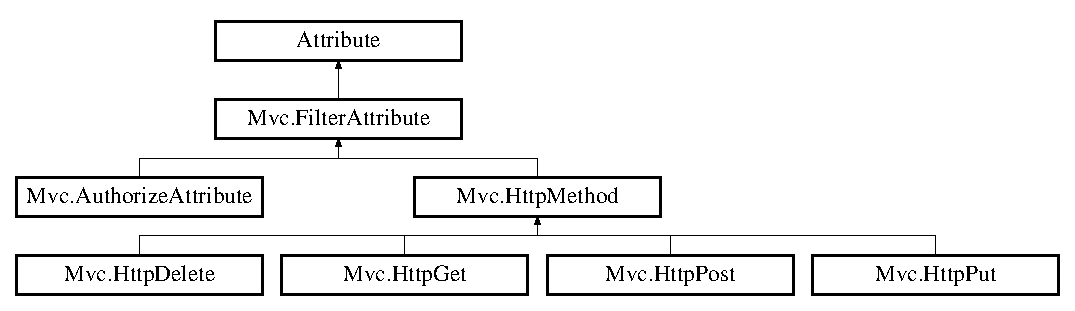
\includegraphics[height=3.733333cm]{class_mvc_1_1_filter_attribute}
\end{center}
\end{figure}


\subsection{Detailed Description}
Representative abstract class of a filter attribute. 



Definition at line 12 of file Filter\+Attribute.\+cs.



The documentation for this class was generated from the following file\+:\begin{DoxyCompactItemize}
\item 
C\+:/\+Users/dieguito12/\+Code/sharpener-\/framework/src/\+Mvc/Filter\+Attribute.\+cs\end{DoxyCompactItemize}

\hypertarget{class_mvc_1_1_http_context}{}\section{Mvc.\+Http\+Context Class Reference}
\label{class_mvc_1_1_http_context}\index{Mvc.\+Http\+Context@{Mvc.\+Http\+Context}}


Representative class of the context information of the http server.  


\subsection*{Properties}
\begin{DoxyCompactItemize}
\item 
Name\+Value\+Collection \hyperlink{class_mvc_1_1_http_context_a353d7d8e5410d7483df18887824d9e03}{Headers}\hspace{0.3cm}{\ttfamily  \mbox{[}get, set\mbox{]}}
\begin{DoxyCompactList}\small\item\em Gets and sets the headers of the response. \end{DoxyCompactList}\item 
string \hyperlink{class_mvc_1_1_http_context_a467051f9750430b364e63069a2327b70}{Session}\hspace{0.3cm}{\ttfamily  \mbox{[}get, set\mbox{]}}
\begin{DoxyCompactList}\small\item\em Gets and sets the session of the app. \end{DoxyCompactList}\item 
\hyperlink{class_mvc_1_1_configuration_manager}{Configuration\+Manager} \hyperlink{class_mvc_1_1_http_context_aa5b6a4fb30772a7739a61b2788b21921}{Configuration\+Manager}\hspace{0.3cm}{\ttfamily  \mbox{[}get, set\mbox{]}}
\begin{DoxyCompactList}\small\item\em Gets a configuration manager. \end{DoxyCompactList}\item 
string \hyperlink{class_mvc_1_1_http_context_afbc78dfac5e1f0097c1a2cf8b9ed63ca}{Physical\+Path}\hspace{0.3cm}{\ttfamily  \mbox{[}get, set\mbox{]}}
\begin{DoxyCompactList}\small\item\em Gets and the physycal path of the app. \end{DoxyCompactList}\end{DoxyCompactItemize}


\subsection{Detailed Description}
Representative class of the context information of the http server. 



Definition at line 13 of file Http\+Context.\+cs.



\subsection{Property Documentation}
\mbox{\Hypertarget{class_mvc_1_1_http_context_aa5b6a4fb30772a7739a61b2788b21921}\label{class_mvc_1_1_http_context_aa5b6a4fb30772a7739a61b2788b21921}} 
\index{Mvc\+::\+Http\+Context@{Mvc\+::\+Http\+Context}!Configuration\+Manager@{Configuration\+Manager}}
\index{Configuration\+Manager@{Configuration\+Manager}!Mvc\+::\+Http\+Context@{Mvc\+::\+Http\+Context}}
\subsubsection{\texorpdfstring{Configuration\+Manager}{ConfigurationManager}}
{\footnotesize\ttfamily \hyperlink{class_mvc_1_1_configuration_manager}{Configuration\+Manager} Mvc.\+Http\+Context.\+Configuration\+Manager\hspace{0.3cm}{\ttfamily [get]}, {\ttfamily [set]}}



Gets a configuration manager. 



Definition at line 69 of file Http\+Context.\+cs.

\mbox{\Hypertarget{class_mvc_1_1_http_context_a353d7d8e5410d7483df18887824d9e03}\label{class_mvc_1_1_http_context_a353d7d8e5410d7483df18887824d9e03}} 
\index{Mvc\+::\+Http\+Context@{Mvc\+::\+Http\+Context}!Headers@{Headers}}
\index{Headers@{Headers}!Mvc\+::\+Http\+Context@{Mvc\+::\+Http\+Context}}
\subsubsection{\texorpdfstring{Headers}{Headers}}
{\footnotesize\ttfamily Name\+Value\+Collection Mvc.\+Http\+Context.\+Headers\hspace{0.3cm}{\ttfamily [get]}, {\ttfamily [set]}}



Gets and sets the headers of the response. 



Definition at line 39 of file Http\+Context.\+cs.

\mbox{\Hypertarget{class_mvc_1_1_http_context_afbc78dfac5e1f0097c1a2cf8b9ed63ca}\label{class_mvc_1_1_http_context_afbc78dfac5e1f0097c1a2cf8b9ed63ca}} 
\index{Mvc\+::\+Http\+Context@{Mvc\+::\+Http\+Context}!Physical\+Path@{Physical\+Path}}
\index{Physical\+Path@{Physical\+Path}!Mvc\+::\+Http\+Context@{Mvc\+::\+Http\+Context}}
\subsubsection{\texorpdfstring{Physical\+Path}{PhysicalPath}}
{\footnotesize\ttfamily string Mvc.\+Http\+Context.\+Physical\+Path\hspace{0.3cm}{\ttfamily [get]}, {\ttfamily [set]}}



Gets and the physycal path of the app. 



Definition at line 84 of file Http\+Context.\+cs.

\mbox{\Hypertarget{class_mvc_1_1_http_context_a467051f9750430b364e63069a2327b70}\label{class_mvc_1_1_http_context_a467051f9750430b364e63069a2327b70}} 
\index{Mvc\+::\+Http\+Context@{Mvc\+::\+Http\+Context}!Session@{Session}}
\index{Session@{Session}!Mvc\+::\+Http\+Context@{Mvc\+::\+Http\+Context}}
\subsubsection{\texorpdfstring{Session}{Session}}
{\footnotesize\ttfamily string Mvc.\+Http\+Context.\+Session\hspace{0.3cm}{\ttfamily [get]}, {\ttfamily [set]}}



Gets and sets the session of the app. 



Definition at line 54 of file Http\+Context.\+cs.



The documentation for this class was generated from the following file\+:\begin{DoxyCompactItemize}
\item 
C\+:/\+Users/dieguito12/\+Code/sharpener-\/framework/src/\+Mvc/Http\+Context.\+cs\end{DoxyCompactItemize}

\hypertarget{class_mvc_1_1_http_delete}{}\section{Mvc.\+Http\+Delete Class Reference}
\label{class_mvc_1_1_http_delete}\index{Mvc.\+Http\+Delete@{Mvc.\+Http\+Delete}}


Representative class of and http D\+E\+L\+E\+TE method attribute  


Inheritance diagram for Mvc.\+Http\+Delete\+:\begin{figure}[H]
\begin{center}
\leavevmode
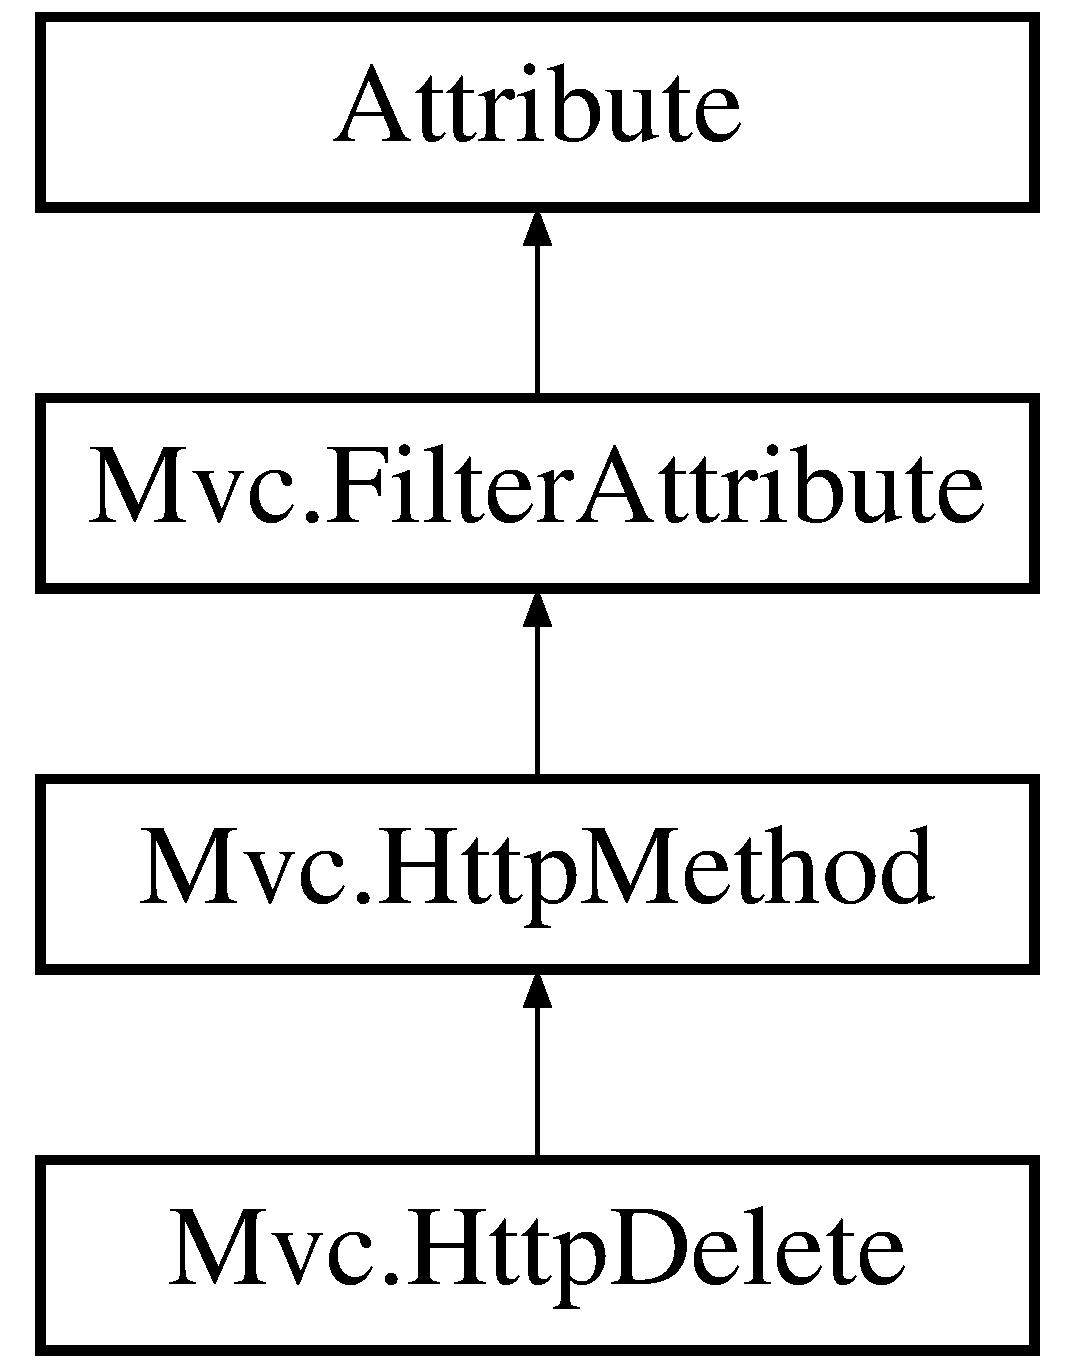
\includegraphics[height=4.000000cm]{class_mvc_1_1_http_delete}
\end{center}
\end{figure}


\subsection{Detailed Description}
Representative class of and http D\+E\+L\+E\+TE method attribute 

Works as a method decorator

Definition at line 54 of file Http\+Method.\+cs.



The documentation for this class was generated from the following file\+:\begin{DoxyCompactItemize}
\item 
C\+:/\+Users/dieguito12/\+Code/sharpener-\/framework/src/\+Mvc/Http\+Method.\+cs\end{DoxyCompactItemize}

\hypertarget{class_mvc_1_1_http_file}{}\section{Mvc.\+Http\+File Class Reference}
\label{class_mvc_1_1_http_file}\index{Mvc.\+Http\+File@{Mvc.\+Http\+File}}


Representative class of a file comming in an http request.  


\subsection*{Public Member Functions}
\begin{DoxyCompactItemize}
\item 
\hyperlink{class_mvc_1_1_http_file_a5a1c81ce7faef7de0719d464196854d6}{Http\+File} (int content\+Length, string content\+Type, string file\+Name, Stream input\+Stream)
\begin{DoxyCompactList}\small\item\em Constructor of the \hyperlink{class_mvc_1_1_http_file}{Http\+File} class. \end{DoxyCompactList}\end{DoxyCompactItemize}
\subsection*{Properties}
\begin{DoxyCompactItemize}
\item 
int \hyperlink{class_mvc_1_1_http_file_a1a279800b9291c4d423de7243a3747ef}{Content\+Length}\hspace{0.3cm}{\ttfamily  \mbox{[}get\mbox{]}}
\begin{DoxyCompactList}\small\item\em Gets the content length of the file. \end{DoxyCompactList}\item 
string \hyperlink{class_mvc_1_1_http_file_aa7581b50f6fa1332ec39995a4a1f71fa}{Content\+Type}\hspace{0.3cm}{\ttfamily  \mbox{[}get\mbox{]}}
\begin{DoxyCompactList}\small\item\em Gets the content type of the file. \end{DoxyCompactList}\item 
string \hyperlink{class_mvc_1_1_http_file_ac87b6e303321d6168c949aa671e8fbab}{File\+Name}\hspace{0.3cm}{\ttfamily  \mbox{[}get\mbox{]}}
\begin{DoxyCompactList}\small\item\em Gets the file name. \end{DoxyCompactList}\item 
Stream \hyperlink{class_mvc_1_1_http_file_aafd93d89d0f3dd9526623810bb55a989}{Input\+Stream}\hspace{0.3cm}{\ttfamily  \mbox{[}get\mbox{]}}
\begin{DoxyCompactList}\small\item\em Gets the data stream of the file. \end{DoxyCompactList}\end{DoxyCompactItemize}


\subsection{Detailed Description}
Representative class of a file comming in an http request. 



Definition at line 13 of file Http\+File.\+cs.



\subsection{Constructor \& Destructor Documentation}
\mbox{\Hypertarget{class_mvc_1_1_http_file_a5a1c81ce7faef7de0719d464196854d6}\label{class_mvc_1_1_http_file_a5a1c81ce7faef7de0719d464196854d6}} 
\index{Mvc\+::\+Http\+File@{Mvc\+::\+Http\+File}!Http\+File@{Http\+File}}
\index{Http\+File@{Http\+File}!Mvc\+::\+Http\+File@{Mvc\+::\+Http\+File}}
\subsubsection{\texorpdfstring{Http\+File()}{HttpFile()}}
{\footnotesize\ttfamily Mvc.\+Http\+File.\+Http\+File (\begin{DoxyParamCaption}\item[{int}]{content\+Length,  }\item[{string}]{content\+Type,  }\item[{string}]{file\+Name,  }\item[{Stream}]{input\+Stream }\end{DoxyParamCaption})}



Constructor of the \hyperlink{class_mvc_1_1_http_file}{Http\+File} class. 


\begin{DoxyParams}{Parameters}
{\em content\+Length} & An int representing the content length of the file.\\
\hline
{\em content\+Type} & A string representing the content type of the file.\\
\hline
{\em file\+Name} & A string representing the file name.\\
\hline
{\em input\+Stream} & A Stream representing the raw information of the file.\\
\hline
\end{DoxyParams}


Definition at line 22 of file Http\+File.\+cs.



\subsection{Property Documentation}
\mbox{\Hypertarget{class_mvc_1_1_http_file_a1a279800b9291c4d423de7243a3747ef}\label{class_mvc_1_1_http_file_a1a279800b9291c4d423de7243a3747ef}} 
\index{Mvc\+::\+Http\+File@{Mvc\+::\+Http\+File}!Content\+Length@{Content\+Length}}
\index{Content\+Length@{Content\+Length}!Mvc\+::\+Http\+File@{Mvc\+::\+Http\+File}}
\subsubsection{\texorpdfstring{Content\+Length}{ContentLength}}
{\footnotesize\ttfamily int Mvc.\+Http\+File.\+Content\+Length\hspace{0.3cm}{\ttfamily [get]}}



Gets the content length of the file. 



Definition at line 38 of file Http\+File.\+cs.

\mbox{\Hypertarget{class_mvc_1_1_http_file_aa7581b50f6fa1332ec39995a4a1f71fa}\label{class_mvc_1_1_http_file_aa7581b50f6fa1332ec39995a4a1f71fa}} 
\index{Mvc\+::\+Http\+File@{Mvc\+::\+Http\+File}!Content\+Type@{Content\+Type}}
\index{Content\+Type@{Content\+Type}!Mvc\+::\+Http\+File@{Mvc\+::\+Http\+File}}
\subsubsection{\texorpdfstring{Content\+Type}{ContentType}}
{\footnotesize\ttfamily string Mvc.\+Http\+File.\+Content\+Type\hspace{0.3cm}{\ttfamily [get]}}



Gets the content type of the file. 



Definition at line 43 of file Http\+File.\+cs.

\mbox{\Hypertarget{class_mvc_1_1_http_file_ac87b6e303321d6168c949aa671e8fbab}\label{class_mvc_1_1_http_file_ac87b6e303321d6168c949aa671e8fbab}} 
\index{Mvc\+::\+Http\+File@{Mvc\+::\+Http\+File}!File\+Name@{File\+Name}}
\index{File\+Name@{File\+Name}!Mvc\+::\+Http\+File@{Mvc\+::\+Http\+File}}
\subsubsection{\texorpdfstring{File\+Name}{FileName}}
{\footnotesize\ttfamily string Mvc.\+Http\+File.\+File\+Name\hspace{0.3cm}{\ttfamily [get]}}



Gets the file name. 



Definition at line 48 of file Http\+File.\+cs.

\mbox{\Hypertarget{class_mvc_1_1_http_file_aafd93d89d0f3dd9526623810bb55a989}\label{class_mvc_1_1_http_file_aafd93d89d0f3dd9526623810bb55a989}} 
\index{Mvc\+::\+Http\+File@{Mvc\+::\+Http\+File}!Input\+Stream@{Input\+Stream}}
\index{Input\+Stream@{Input\+Stream}!Mvc\+::\+Http\+File@{Mvc\+::\+Http\+File}}
\subsubsection{\texorpdfstring{Input\+Stream}{InputStream}}
{\footnotesize\ttfamily Stream Mvc.\+Http\+File.\+Input\+Stream\hspace{0.3cm}{\ttfamily [get]}}



Gets the data stream of the file. 



Definition at line 53 of file Http\+File.\+cs.



The documentation for this class was generated from the following file\+:\begin{DoxyCompactItemize}
\item 
C\+:/\+Users/dieguito12/\+Code/sharpener-\/framework/src/\+Mvc/Http\+File.\+cs\end{DoxyCompactItemize}

\hypertarget{class_mvc_1_1_http_get}{}\section{Mvc.\+Http\+Get Class Reference}
\label{class_mvc_1_1_http_get}\index{Mvc.\+Http\+Get@{Mvc.\+Http\+Get}}


Representative class of and http G\+ET method attribute  


Inheritance diagram for Mvc.\+Http\+Get\+:\begin{figure}[H]
\begin{center}
\leavevmode
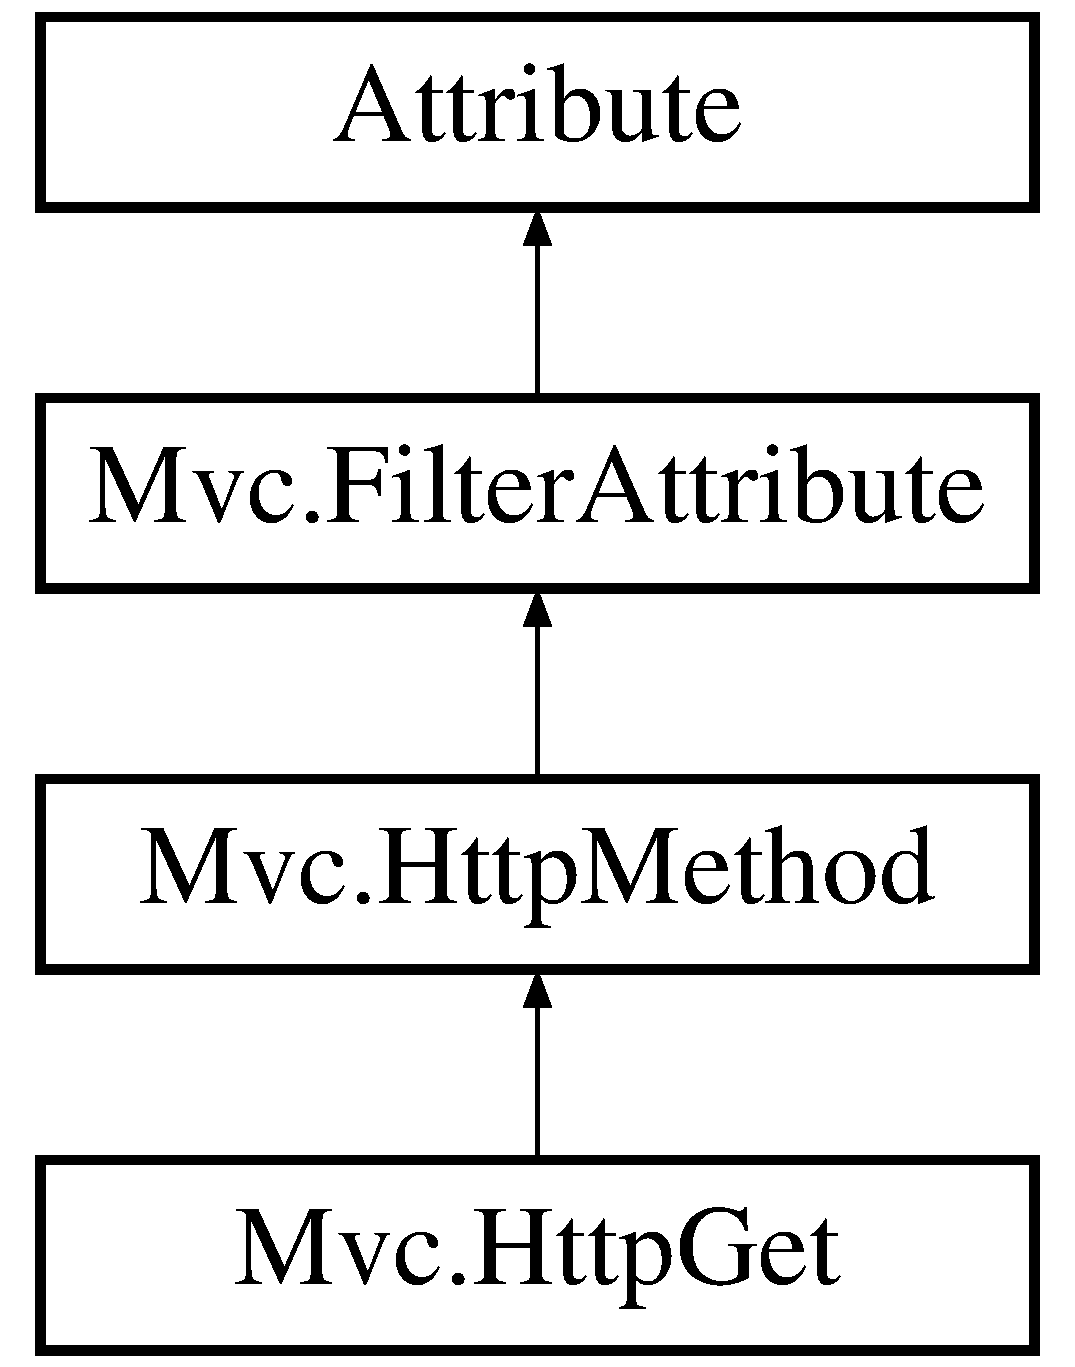
\includegraphics[height=4.000000cm]{class_mvc_1_1_http_get}
\end{center}
\end{figure}


\subsection{Detailed Description}
Representative class of and http G\+ET method attribute 

Works as a method decorator

Definition at line 34 of file Http\+Method.\+cs.



The documentation for this class was generated from the following file\+:\begin{DoxyCompactItemize}
\item 
C\+:/\+Users/dieguito12/\+Code/sharpener-\/framework/src/\+Mvc/Http\+Method.\+cs\end{DoxyCompactItemize}

\hypertarget{class_mvc_1_1_http_method}{}\section{Mvc.\+Http\+Method Class Reference}
\label{class_mvc_1_1_http_method}\index{Mvc.\+Http\+Method@{Mvc.\+Http\+Method}}


Representative class of and http method attribute  


Inheritance diagram for Mvc.\+Http\+Method\+:\begin{figure}[H]
\begin{center}
\leavevmode
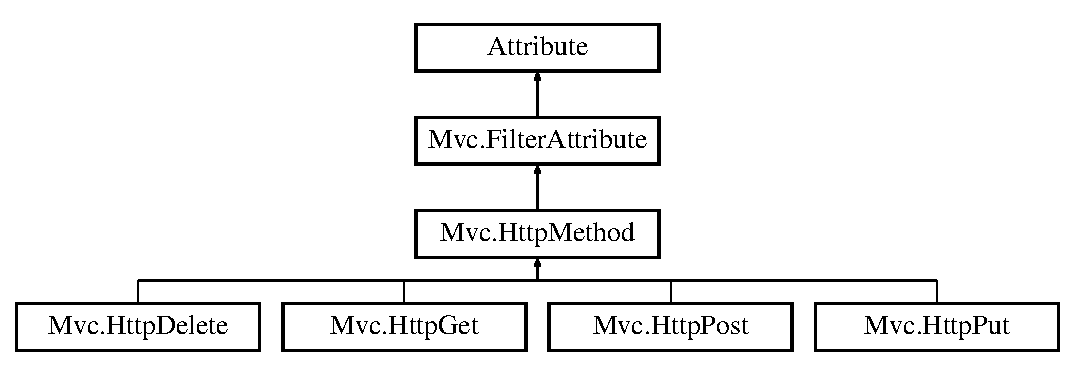
\includegraphics[height=4.000000cm]{class_mvc_1_1_http_method}
\end{center}
\end{figure}


\subsection{Detailed Description}
Representative class of and http method attribute 

Works as a method decorator

Definition at line 14 of file Http\+Method.\+cs.



The documentation for this class was generated from the following file\+:\begin{DoxyCompactItemize}
\item 
C\+:/\+Users/dieguito12/\+Code/sharpener-\/framework/src/\+Mvc/Http\+Method.\+cs\end{DoxyCompactItemize}

\hypertarget{class_mvc_1_1_http_post}{}\section{Mvc.\+Http\+Post Class Reference}
\label{class_mvc_1_1_http_post}\index{Mvc.\+Http\+Post@{Mvc.\+Http\+Post}}


Representative class of and http P\+O\+ST method attribute  


Inheritance diagram for Mvc.\+Http\+Post\+:\begin{figure}[H]
\begin{center}
\leavevmode
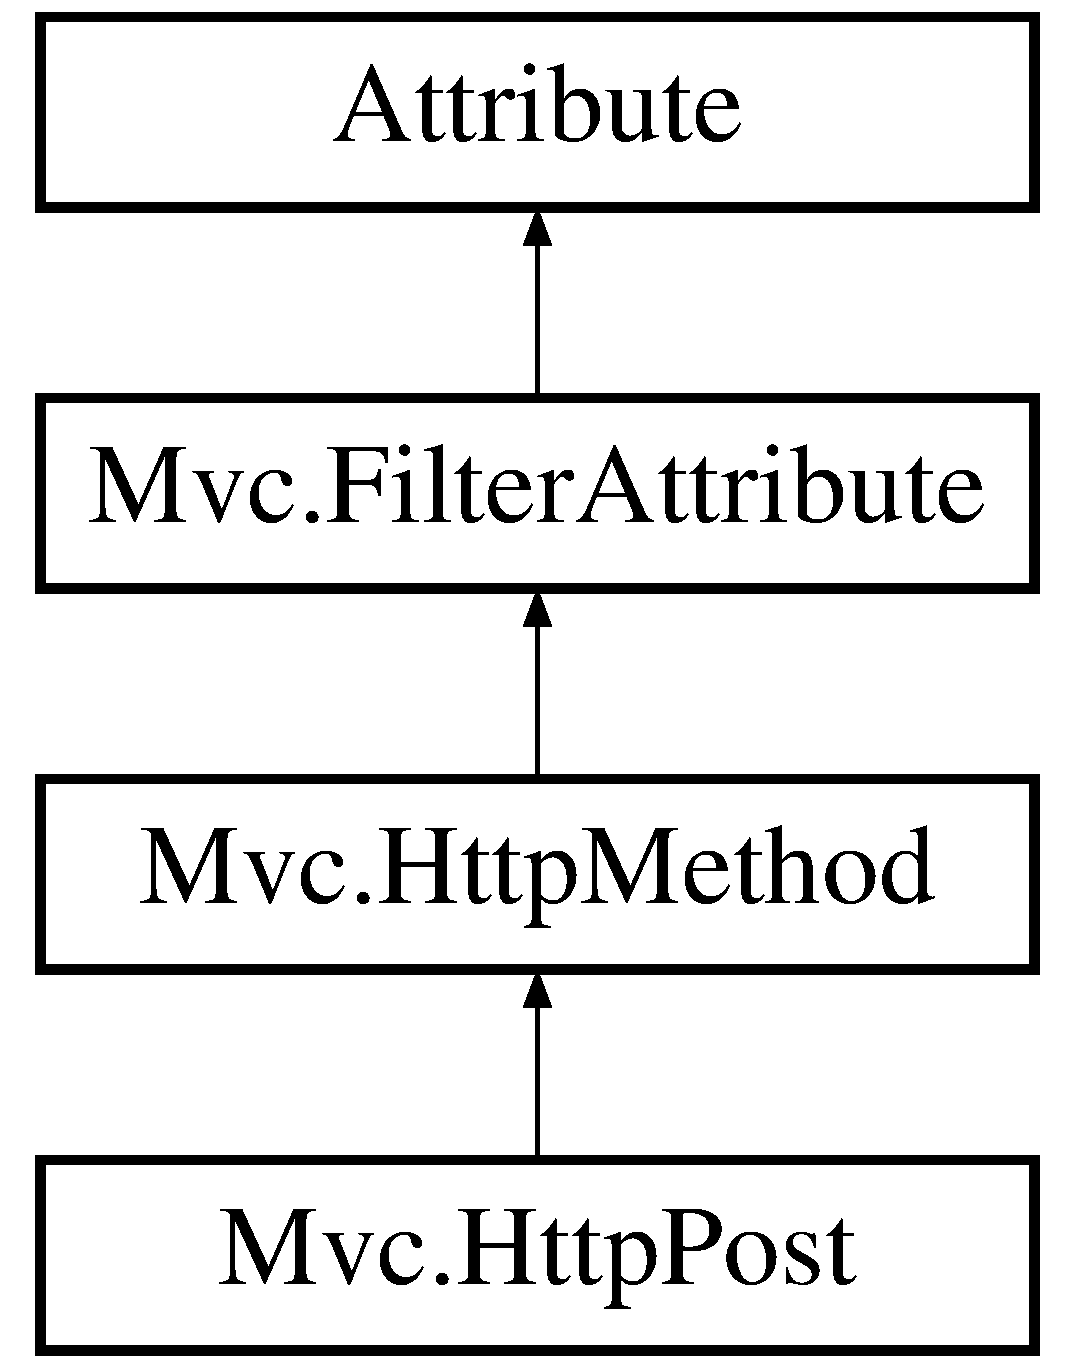
\includegraphics[height=4.000000cm]{class_mvc_1_1_http_post}
\end{center}
\end{figure}


\subsection{Detailed Description}
Representative class of and http P\+O\+ST method attribute 

Works as a method decorator

Definition at line 24 of file Http\+Method.\+cs.



The documentation for this class was generated from the following file\+:\begin{DoxyCompactItemize}
\item 
C\+:/\+Users/dieguito12/\+Code/sharpener-\/framework/src/\+Mvc/Http\+Method.\+cs\end{DoxyCompactItemize}

\hypertarget{class_mvc_1_1_http_put}{}\section{Mvc.\+Http\+Put Class Reference}
\label{class_mvc_1_1_http_put}\index{Mvc.\+Http\+Put@{Mvc.\+Http\+Put}}


Representative class of and http P\+UT method attribute  


Inheritance diagram for Mvc.\+Http\+Put\+:\begin{figure}[H]
\begin{center}
\leavevmode
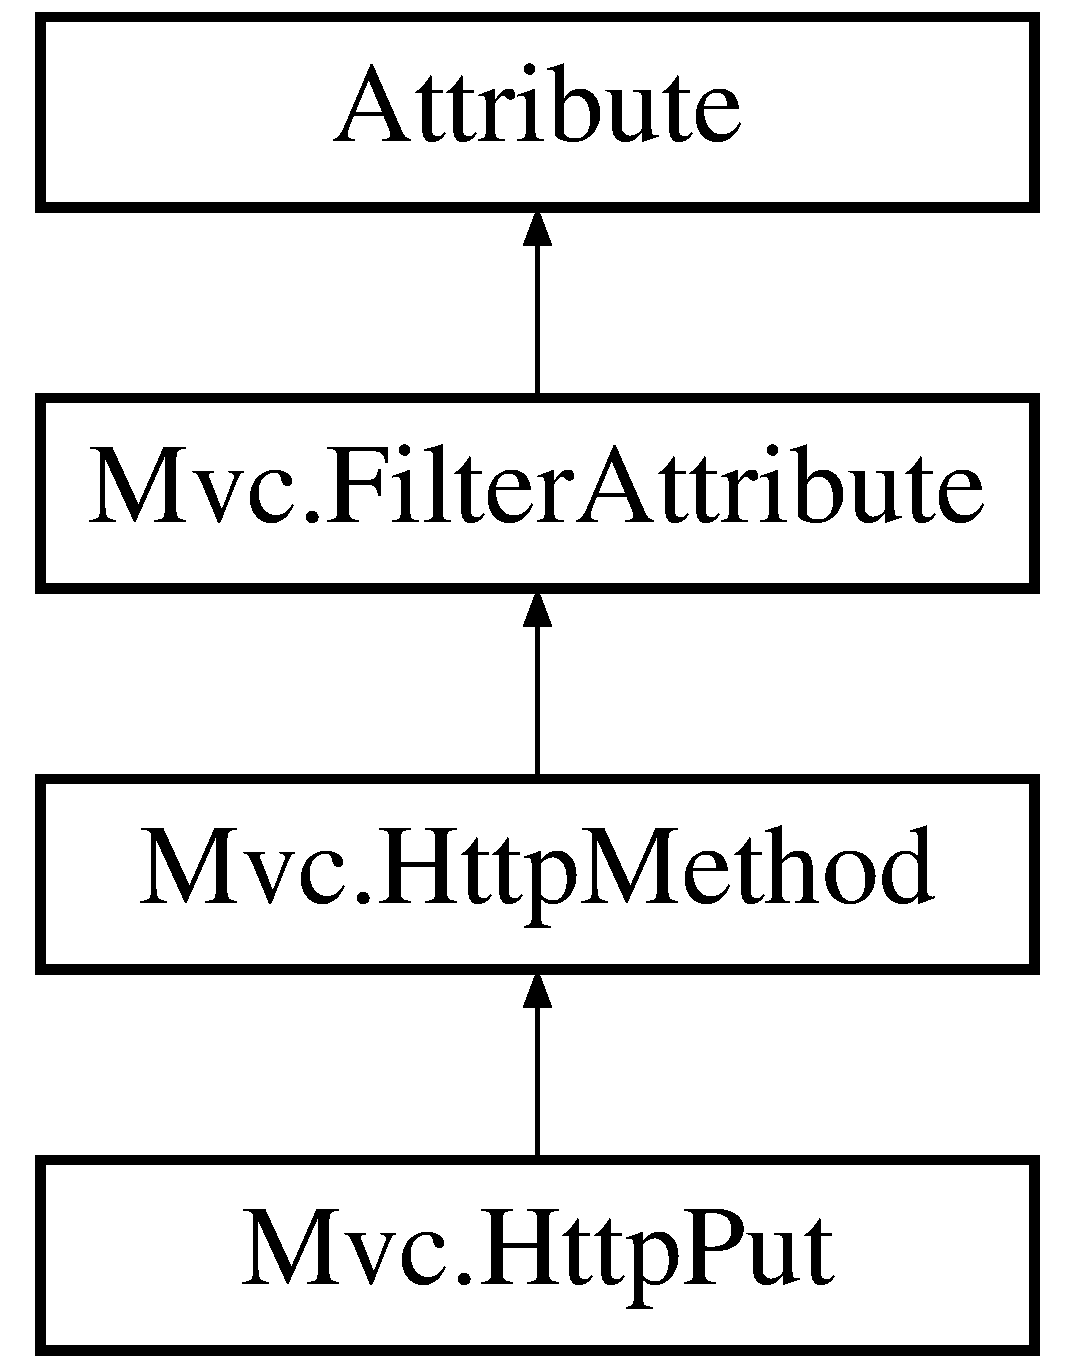
\includegraphics[height=4.000000cm]{class_mvc_1_1_http_put}
\end{center}
\end{figure}


\subsection{Detailed Description}
Representative class of and http P\+UT method attribute 

Works as a method decorator

Definition at line 44 of file Http\+Method.\+cs.



The documentation for this class was generated from the following file\+:\begin{DoxyCompactItemize}
\item 
C\+:/\+Users/dieguito12/\+Code/sharpener-\/framework/src/\+Mvc/Http\+Method.\+cs\end{DoxyCompactItemize}

\hypertarget{interface_mvc_1_1_i_action_result}{}\section{Mvc.\+I\+Action\+Result Interface Reference}
\label{interface_mvc_1_1_i_action_result}\index{Mvc.\+I\+Action\+Result@{Mvc.\+I\+Action\+Result}}


Representative interface of the result of a Controller  


Inheritance diagram for Mvc.\+I\+Action\+Result\+:\begin{figure}[H]
\begin{center}
\leavevmode
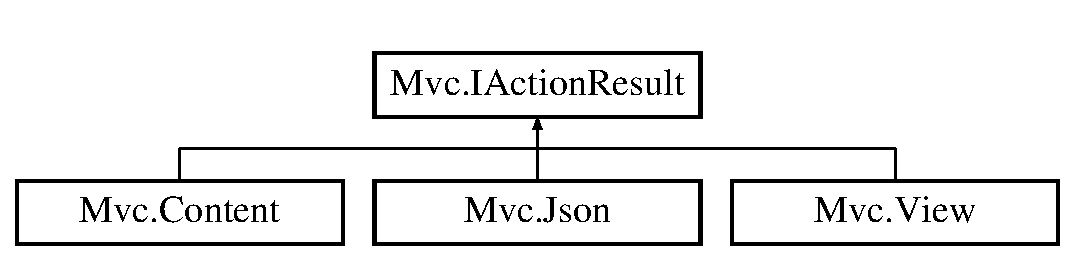
\includegraphics[height=2.000000cm]{interface_mvc_1_1_i_action_result}
\end{center}
\end{figure}
\subsection*{Public Member Functions}
\begin{DoxyCompactItemize}
\item 
Memory\+Stream \hyperlink{interface_mvc_1_1_i_action_result_a7cf7423071384c7b2bac75a5f4d6e25c}{Response} ()
\begin{DoxyCompactList}\small\item\em Gets the response of the controller in a stream. \end{DoxyCompactList}\item 
string \hyperlink{interface_mvc_1_1_i_action_result_a8ad08f29bba90dfbe06d7a00465af10a}{Content\+Type} ()
\begin{DoxyCompactList}\small\item\em Gets the content type of the response. \end{DoxyCompactList}\item 
int \hyperlink{interface_mvc_1_1_i_action_result_ab6b85ae50597587395df99b972c3d26b}{Code} ()
\begin{DoxyCompactList}\small\item\em Gets the status code of the response. \end{DoxyCompactList}\item 
string \hyperlink{interface_mvc_1_1_i_action_result_a036707da116ea300eae90e105b8d1ced}{Redirection} ()
\begin{DoxyCompactList}\small\item\em Gets the url where the response is going to redirect (if there is any). \end{DoxyCompactList}\end{DoxyCompactItemize}


\subsection{Detailed Description}
Representative interface of the result of a Controller 



Definition at line 13 of file Action\+Result.\+cs.



\subsection{Member Function Documentation}
\mbox{\Hypertarget{interface_mvc_1_1_i_action_result_ab6b85ae50597587395df99b972c3d26b}\label{interface_mvc_1_1_i_action_result_ab6b85ae50597587395df99b972c3d26b}} 
\index{Mvc\+::\+I\+Action\+Result@{Mvc\+::\+I\+Action\+Result}!Code@{Code}}
\index{Code@{Code}!Mvc\+::\+I\+Action\+Result@{Mvc\+::\+I\+Action\+Result}}
\subsubsection{\texorpdfstring{Code()}{Code()}}
{\footnotesize\ttfamily int Mvc.\+I\+Action\+Result.\+Code (\begin{DoxyParamCaption}{ }\end{DoxyParamCaption})}



Gets the status code of the response. 

\begin{DoxyReturn}{Returns}
An int representing the status code
\end{DoxyReturn}


Implemented in \hyperlink{class_mvc_1_1_json_aab9ce2b098ce0b4bfe8ad835a33e71d5}{Mvc.\+Json}, \hyperlink{class_mvc_1_1_view_a7e723a9bafb2f876175d1396c06da062}{Mvc.\+View}, and \hyperlink{class_mvc_1_1_content_a77175a25c002834c59e14cde60719c28}{Mvc.\+Content}.

\mbox{\Hypertarget{interface_mvc_1_1_i_action_result_a8ad08f29bba90dfbe06d7a00465af10a}\label{interface_mvc_1_1_i_action_result_a8ad08f29bba90dfbe06d7a00465af10a}} 
\index{Mvc\+::\+I\+Action\+Result@{Mvc\+::\+I\+Action\+Result}!Content\+Type@{Content\+Type}}
\index{Content\+Type@{Content\+Type}!Mvc\+::\+I\+Action\+Result@{Mvc\+::\+I\+Action\+Result}}
\subsubsection{\texorpdfstring{Content\+Type()}{ContentType()}}
{\footnotesize\ttfamily string Mvc.\+I\+Action\+Result.\+Content\+Type (\begin{DoxyParamCaption}{ }\end{DoxyParamCaption})}



Gets the content type of the response. 

\begin{DoxyReturn}{Returns}
A string representing the content type of the response
\end{DoxyReturn}


Implemented in \hyperlink{class_mvc_1_1_json_aa2572df4640e171276244cbb14070284}{Mvc.\+Json}, \hyperlink{class_mvc_1_1_view_a0b14b3b8e85c97ada45a32dfcc30f157}{Mvc.\+View}, and \hyperlink{class_mvc_1_1_content_a5d384ef7d466dfc88ccf1eb7f10728ad}{Mvc.\+Content}.

\mbox{\Hypertarget{interface_mvc_1_1_i_action_result_a036707da116ea300eae90e105b8d1ced}\label{interface_mvc_1_1_i_action_result_a036707da116ea300eae90e105b8d1ced}} 
\index{Mvc\+::\+I\+Action\+Result@{Mvc\+::\+I\+Action\+Result}!Redirection@{Redirection}}
\index{Redirection@{Redirection}!Mvc\+::\+I\+Action\+Result@{Mvc\+::\+I\+Action\+Result}}
\subsubsection{\texorpdfstring{Redirection()}{Redirection()}}
{\footnotesize\ttfamily string Mvc.\+I\+Action\+Result.\+Redirection (\begin{DoxyParamCaption}{ }\end{DoxyParamCaption})}



Gets the url where the response is going to redirect (if there is any). 

\begin{DoxyReturn}{Returns}
A string representing the redirection url
\end{DoxyReturn}


Implemented in \hyperlink{class_mvc_1_1_json_af8cd874b2a4c9692f0200bde97d40c87}{Mvc.\+Json}, \hyperlink{class_mvc_1_1_view_a6628a16ae93e0269d91413a3a38d0132}{Mvc.\+View}, and \hyperlink{class_mvc_1_1_content_ae4eba27dbea637dc61bc4b681f731545}{Mvc.\+Content}.

\mbox{\Hypertarget{interface_mvc_1_1_i_action_result_a7cf7423071384c7b2bac75a5f4d6e25c}\label{interface_mvc_1_1_i_action_result_a7cf7423071384c7b2bac75a5f4d6e25c}} 
\index{Mvc\+::\+I\+Action\+Result@{Mvc\+::\+I\+Action\+Result}!Response@{Response}}
\index{Response@{Response}!Mvc\+::\+I\+Action\+Result@{Mvc\+::\+I\+Action\+Result}}
\subsubsection{\texorpdfstring{Response()}{Response()}}
{\footnotesize\ttfamily Memory\+Stream Mvc.\+I\+Action\+Result.\+Response (\begin{DoxyParamCaption}{ }\end{DoxyParamCaption})}



Gets the response of the controller in a stream. 

\begin{DoxyReturn}{Returns}
Memory\+Stream that represents the response of the controller.
\end{DoxyReturn}


Implemented in \hyperlink{class_mvc_1_1_json_ae94043bfe0049a44c8b0c61a13b61ac9}{Mvc.\+Json}, \hyperlink{class_mvc_1_1_view_a8a5a1a1990be0c3704b4f3262c503a2a}{Mvc.\+View}, and \hyperlink{class_mvc_1_1_content_aabe147bc684eed8af000906fbfe92b61}{Mvc.\+Content}.



The documentation for this interface was generated from the following file\+:\begin{DoxyCompactItemize}
\item 
C\+:/\+Users/dieguito12/\+Code/sharpener-\/framework/src/\+Mvc/Action\+Result.\+cs\end{DoxyCompactItemize}

\hypertarget{class_mvc_1_1_json}{}\section{Mvc.\+Json Class Reference}
\label{class_mvc_1_1_json}\index{Mvc.\+Json@{Mvc.\+Json}}


Representative class of a json response  


Inheritance diagram for Mvc.\+Json\+:\begin{figure}[H]
\begin{center}
\leavevmode
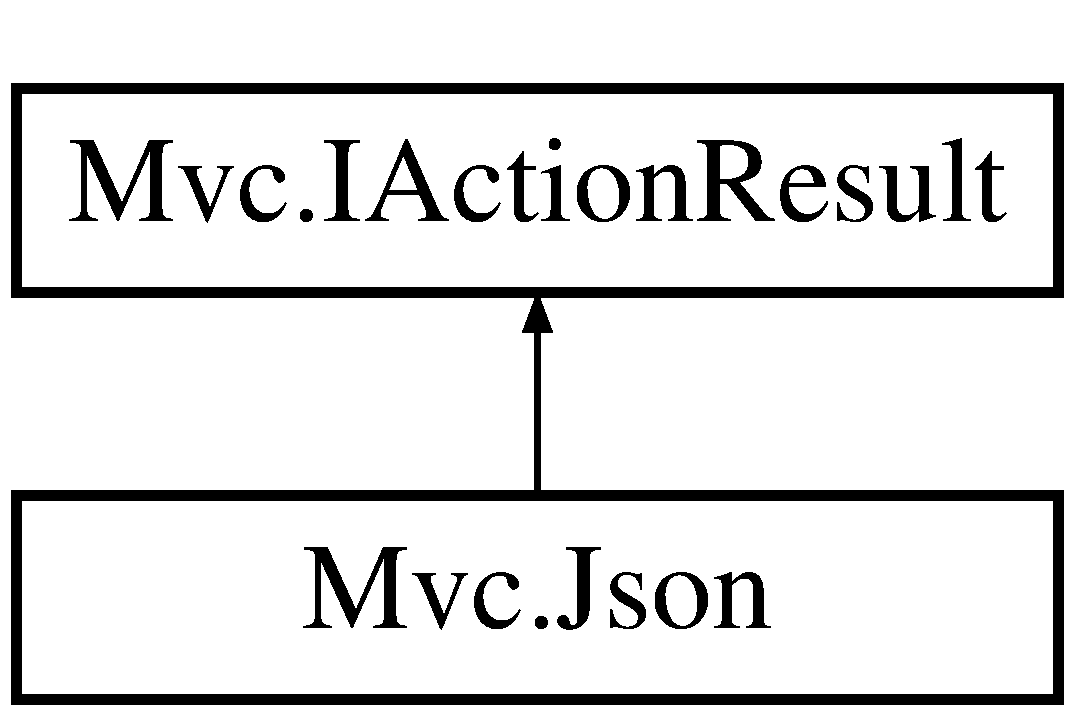
\includegraphics[height=2.000000cm]{class_mvc_1_1_json}
\end{center}
\end{figure}
\subsection*{Public Member Functions}
\begin{DoxyCompactItemize}
\item 
\hyperlink{class_mvc_1_1_json_a0b86fdb1b35bca88ae21f0f2282a710d}{Json} (string json, int code)
\begin{DoxyCompactList}\small\item\em Constructor of the \hyperlink{class_mvc_1_1_json}{Json} class. \end{DoxyCompactList}\item 
Memory\+Stream \hyperlink{class_mvc_1_1_json_ae94043bfe0049a44c8b0c61a13b61ac9}{Response} ()
\begin{DoxyCompactList}\small\item\em Gets the response of the controller in a stream. \end{DoxyCompactList}\item 
int \hyperlink{class_mvc_1_1_json_aab9ce2b098ce0b4bfe8ad835a33e71d5}{Code} ()
\begin{DoxyCompactList}\small\item\em Gets the status code of the response. \end{DoxyCompactList}\item 
string \hyperlink{class_mvc_1_1_json_aa2572df4640e171276244cbb14070284}{Content\+Type} ()
\begin{DoxyCompactList}\small\item\em Gets the content type of the response. \end{DoxyCompactList}\item 
string \hyperlink{class_mvc_1_1_json_af8cd874b2a4c9692f0200bde97d40c87}{Redirection} ()
\begin{DoxyCompactList}\small\item\em Gets the url where the response is going to redirect (if there is any). \end{DoxyCompactList}\end{DoxyCompactItemize}
\subsection*{Static Public Member Functions}
\begin{DoxyCompactItemize}
\item 
static string \hyperlink{class_mvc_1_1_json_a7f2eac02ea84b7b0c9c277d54e347c8a}{Jsonify} (Name\+Value\+Collection values)
\begin{DoxyCompactList}\small\item\em An static method that turns a Name\+Value\+Collection into a json string. \end{DoxyCompactList}\item 
static Name\+Value\+Collection \hyperlink{class_mvc_1_1_json_a6876cfad310dbe0a704204bec09c9d66}{Serialize} (string json)
\begin{DoxyCompactList}\small\item\em An static method that turns a json string into a Name\+Value\+Collection. \end{DoxyCompactList}\end{DoxyCompactItemize}


\subsection{Detailed Description}
Representative class of a json response 



Definition at line 16 of file Json.\+cs.



\subsection{Constructor \& Destructor Documentation}
\mbox{\Hypertarget{class_mvc_1_1_json_a0b86fdb1b35bca88ae21f0f2282a710d}\label{class_mvc_1_1_json_a0b86fdb1b35bca88ae21f0f2282a710d}} 
\index{Mvc\+::\+Json@{Mvc\+::\+Json}!Json@{Json}}
\index{Json@{Json}!Mvc\+::\+Json@{Mvc\+::\+Json}}
\subsubsection{\texorpdfstring{Json()}{Json()}}
{\footnotesize\ttfamily Mvc.\+Json.\+Json (\begin{DoxyParamCaption}\item[{string}]{json,  }\item[{int}]{code }\end{DoxyParamCaption})}



Constructor of the \hyperlink{class_mvc_1_1_json}{Json} class. 


\begin{DoxyParams}{Parameters}
{\em json} & A string representing the json to respond.\\
\hline
{\em code} & An int representing the status code.\\
\hline
\end{DoxyParams}


Definition at line 70 of file Json.\+cs.



\subsection{Member Function Documentation}
\mbox{\Hypertarget{class_mvc_1_1_json_aab9ce2b098ce0b4bfe8ad835a33e71d5}\label{class_mvc_1_1_json_aab9ce2b098ce0b4bfe8ad835a33e71d5}} 
\index{Mvc\+::\+Json@{Mvc\+::\+Json}!Code@{Code}}
\index{Code@{Code}!Mvc\+::\+Json@{Mvc\+::\+Json}}
\subsubsection{\texorpdfstring{Code()}{Code()}}
{\footnotesize\ttfamily int Mvc.\+Json.\+Code (\begin{DoxyParamCaption}{ }\end{DoxyParamCaption})}



Gets the status code of the response. 

\begin{DoxyReturn}{Returns}
An int representing the status code
\end{DoxyReturn}


Implements \hyperlink{interface_mvc_1_1_i_action_result_ab6b85ae50597587395df99b972c3d26b}{Mvc.\+I\+Action\+Result}.



Definition at line 90 of file Json.\+cs.

\mbox{\Hypertarget{class_mvc_1_1_json_aa2572df4640e171276244cbb14070284}\label{class_mvc_1_1_json_aa2572df4640e171276244cbb14070284}} 
\index{Mvc\+::\+Json@{Mvc\+::\+Json}!Content\+Type@{Content\+Type}}
\index{Content\+Type@{Content\+Type}!Mvc\+::\+Json@{Mvc\+::\+Json}}
\subsubsection{\texorpdfstring{Content\+Type()}{ContentType()}}
{\footnotesize\ttfamily string Mvc.\+Json.\+Content\+Type (\begin{DoxyParamCaption}{ }\end{DoxyParamCaption})}



Gets the content type of the response. 

\begin{DoxyReturn}{Returns}
A string representing the content type of the response
\end{DoxyReturn}


Implements \hyperlink{interface_mvc_1_1_i_action_result_a8ad08f29bba90dfbe06d7a00465af10a}{Mvc.\+I\+Action\+Result}.



Definition at line 99 of file Json.\+cs.

\mbox{\Hypertarget{class_mvc_1_1_json_a7f2eac02ea84b7b0c9c277d54e347c8a}\label{class_mvc_1_1_json_a7f2eac02ea84b7b0c9c277d54e347c8a}} 
\index{Mvc\+::\+Json@{Mvc\+::\+Json}!Jsonify@{Jsonify}}
\index{Jsonify@{Jsonify}!Mvc\+::\+Json@{Mvc\+::\+Json}}
\subsubsection{\texorpdfstring{Jsonify()}{Jsonify()}}
{\footnotesize\ttfamily static string Mvc.\+Json.\+Jsonify (\begin{DoxyParamCaption}\item[{Name\+Value\+Collection}]{values }\end{DoxyParamCaption})\hspace{0.3cm}{\ttfamily [static]}}



An static method that turns a Name\+Value\+Collection into a json string. 


\begin{DoxyParams}{Parameters}
{\em values} & Name\+Value\+Collection with the json values\\
\hline
\end{DoxyParams}
\begin{DoxyReturn}{Returns}
A string representing a json.
\end{DoxyReturn}


Definition at line 33 of file Json.\+cs.

\mbox{\Hypertarget{class_mvc_1_1_json_af8cd874b2a4c9692f0200bde97d40c87}\label{class_mvc_1_1_json_af8cd874b2a4c9692f0200bde97d40c87}} 
\index{Mvc\+::\+Json@{Mvc\+::\+Json}!Redirection@{Redirection}}
\index{Redirection@{Redirection}!Mvc\+::\+Json@{Mvc\+::\+Json}}
\subsubsection{\texorpdfstring{Redirection()}{Redirection()}}
{\footnotesize\ttfamily string Mvc.\+Json.\+Redirection (\begin{DoxyParamCaption}{ }\end{DoxyParamCaption})}



Gets the url where the response is going to redirect (if there is any). 

\begin{DoxyReturn}{Returns}
A string representing the redirection url
\end{DoxyReturn}


Implements \hyperlink{interface_mvc_1_1_i_action_result_a036707da116ea300eae90e105b8d1ced}{Mvc.\+I\+Action\+Result}.



Definition at line 108 of file Json.\+cs.

\mbox{\Hypertarget{class_mvc_1_1_json_ae94043bfe0049a44c8b0c61a13b61ac9}\label{class_mvc_1_1_json_ae94043bfe0049a44c8b0c61a13b61ac9}} 
\index{Mvc\+::\+Json@{Mvc\+::\+Json}!Response@{Response}}
\index{Response@{Response}!Mvc\+::\+Json@{Mvc\+::\+Json}}
\subsubsection{\texorpdfstring{Response()}{Response()}}
{\footnotesize\ttfamily Memory\+Stream Mvc.\+Json.\+Response (\begin{DoxyParamCaption}{ }\end{DoxyParamCaption})}



Gets the response of the controller in a stream. 

\begin{DoxyReturn}{Returns}
Memory\+Stream that represents the response of the controller.
\end{DoxyReturn}


Implements \hyperlink{interface_mvc_1_1_i_action_result_a7cf7423071384c7b2bac75a5f4d6e25c}{Mvc.\+I\+Action\+Result}.



Definition at line 80 of file Json.\+cs.

\mbox{\Hypertarget{class_mvc_1_1_json_a6876cfad310dbe0a704204bec09c9d66}\label{class_mvc_1_1_json_a6876cfad310dbe0a704204bec09c9d66}} 
\index{Mvc\+::\+Json@{Mvc\+::\+Json}!Serialize@{Serialize}}
\index{Serialize@{Serialize}!Mvc\+::\+Json@{Mvc\+::\+Json}}
\subsubsection{\texorpdfstring{Serialize()}{Serialize()}}
{\footnotesize\ttfamily static Name\+Value\+Collection Mvc.\+Json.\+Serialize (\begin{DoxyParamCaption}\item[{string}]{json }\end{DoxyParamCaption})\hspace{0.3cm}{\ttfamily [static]}}



An static method that turns a json string into a Name\+Value\+Collection. 


\begin{DoxyParams}{Parameters}
{\em json} & A string representing a json\\
\hline
\end{DoxyParams}
\begin{DoxyReturn}{Returns}
A Name\+Value\+Collection with the json data.
\end{DoxyReturn}


Definition at line 54 of file Json.\+cs.



The documentation for this class was generated from the following file\+:\begin{DoxyCompactItemize}
\item 
C\+:/\+Users/dieguito12/\+Code/sharpener-\/framework/src/\+Mvc/Json.\+cs\end{DoxyCompactItemize}

\hypertarget{class_mvc_1_1_p_http_application}{}\section{Mvc.\+P\+Http\+Application Class Reference}
\label{class_mvc_1_1_p_http_application}\index{Mvc.\+P\+Http\+Application@{Mvc.\+P\+Http\+Application}}


Interface of a Http application hosted in our Web Server.  


Inheritance diagram for Mvc.\+P\+Http\+Application\+:\begin{figure}[H]
\begin{center}
\leavevmode
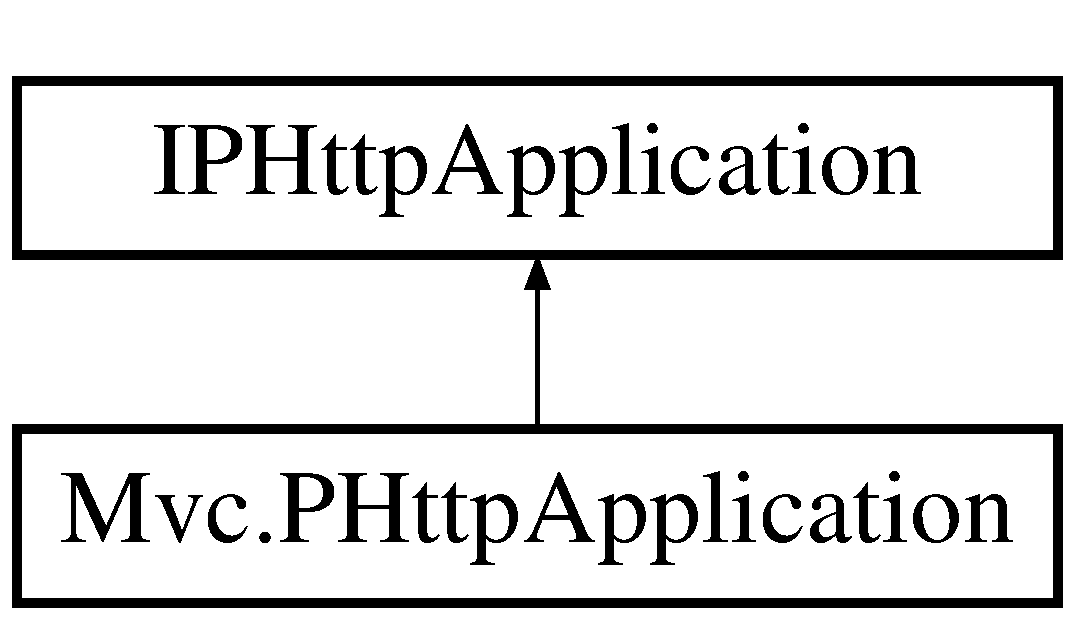
\includegraphics[height=2.000000cm]{class_mvc_1_1_p_http_application}
\end{center}
\end{figure}
\subsection*{Public Member Functions}
\begin{DoxyCompactItemize}
\item 
Name\+Value\+Collection \hyperlink{class_mvc_1_1_p_http_application_ae520dc0bf0c265e6c7114d918f9aa6a0}{Get\+Headers} ()
\begin{DoxyCompactList}\small\item\em Gets the headers of the app response to the web server \end{DoxyCompactList}\item 
\hyperlink{class_mvc_1_1_p_http_application_afea25215430e7e6346ba122a10693ed1}{P\+Http\+Application} ()
\begin{DoxyCompactList}\small\item\em Constructor of the \hyperlink{class_mvc_1_1_p_http_application}{P\+Http\+Application} class. \end{DoxyCompactList}\item 
void \hyperlink{class_mvc_1_1_p_http_application_a3a4aae05eadf7da66bdd37f96c48f79f}{Register\+Routing\+Map} (string routing\+Map)
\begin{DoxyCompactList}\small\item\em Registers the routing map pattern \end{DoxyCompactList}\item 
void \hyperlink{class_mvc_1_1_p_http_application_a79ba7ef50171a93e565f46d5e19ae019}{Init} (string name, string virtual\+Path, string physical\+Path)
\begin{DoxyCompactList}\small\item\em Initializes the application. \end{DoxyCompactList}\item 
string \hyperlink{class_mvc_1_1_p_http_application_acb04996af75e14fdfdc1dcacf7a52247}{Error} (string path, string error\+Message)
\begin{DoxyCompactList}\small\item\em Returns an error page given the path of the template and the error message \end{DoxyCompactList}\item 
void \hyperlink{class_mvc_1_1_p_http_application_a38a4aec623c570fbd05c9e4c33951a05}{On\+Application\+Start} (string physical\+Path)
\begin{DoxyCompactList}\small\item\em Listener of the application start event \end{DoxyCompactList}\item 
void \hyperlink{class_mvc_1_1_p_http_application_af4ab5d8d6f1db0a740617bd686fd0e4a}{On\+Pre\+Application\+Start} (string virtual\+Path)
\begin{DoxyCompactList}\small\item\em Listener of the pre application start event. \end{DoxyCompactList}\item 
object \hyperlink{class_mvc_1_1_p_http_application_a9dc63c8a87637cf4ffdf3ec78f3261a2}{Get\+Configuration\+Manager} ()
\begin{DoxyCompactList}\small\item\em Gets the configuration manager as a generic object \end{DoxyCompactList}\item 
string \hyperlink{class_mvc_1_1_p_http_application_a4970faea54350be3fb4575014f7b58ec}{Get\+Session} ()
\begin{DoxyCompactList}\small\item\em Gets the current session of the application. \end{DoxyCompactList}\item 
object \hyperlink{class_mvc_1_1_p_http_application_a4de3706c2afcbfb56c98a7ca820f53a7}{Execute\+Controller\+Action} (Dictionary$<$ string, object $>$ action\+To\+Call)
\begin{DoxyCompactList}\small\item\em Executes an action of a controller \end{DoxyCompactList}\item 
object \hyperlink{class_mvc_1_1_p_http_application_a9497e9f68b567946aa16f67c9536bb21}{Clone} ()
\begin{DoxyCompactList}\small\item\em Clones this object \end{DoxyCompactList}\end{DoxyCompactItemize}
\subsection*{Properties}
\begin{DoxyCompactItemize}
\item 
Name\+Value\+Collection \hyperlink{class_mvc_1_1_p_http_application_aafb61bb03731b040d45a8dab426132fd}{Headers}\hspace{0.3cm}{\ttfamily  \mbox{[}get\mbox{]}}
\begin{DoxyCompactList}\small\item\em Gets the headers of the app response to the web server \end{DoxyCompactList}\item 
string \hyperlink{class_mvc_1_1_p_http_application_a6b88e2d6ba56c3e26558310ef17a329d}{Configuration\+Path}\hspace{0.3cm}{\ttfamily  \mbox{[}get, protected set\mbox{]}}
\begin{DoxyCompactList}\small\item\em Gets the path of the application configuration file. \end{DoxyCompactList}\item 
string \hyperlink{class_mvc_1_1_p_http_application_a49f7f8b5103b1141ab11b0e482af51fa}{Name}\hspace{0.3cm}{\ttfamily  \mbox{[}get, set\mbox{]}}
\begin{DoxyCompactList}\small\item\em Gets the name of the application.\end{DoxyCompactList}\item 
string \hyperlink{class_mvc_1_1_p_http_application_acc2f12d716e578beb22a506aaf614491}{Physical\+Path}\hspace{0.3cm}{\ttfamily  \mbox{[}get, set\mbox{]}}
\begin{DoxyCompactList}\small\item\em Gets the physical path of the application dll. \end{DoxyCompactList}\item 
string \hyperlink{class_mvc_1_1_p_http_application_a51d755edd9a7c81e6173730c75eae430}{Virtual\+Path}\hspace{0.3cm}{\ttfamily  \mbox{[}get, set\mbox{]}}
\begin{DoxyCompactList}\small\item\em Gets or sets the virtual path of the application.\end{DoxyCompactList}\item 
\hyperlink{class_mvc_1_1_configuration_manager}{Configuration\+Manager} \hyperlink{class_mvc_1_1_p_http_application_a19b5b22d6422a32d76b113fecda86d88}{Configuration\+Manager}\hspace{0.3cm}{\ttfamily  \mbox{[}get\mbox{]}}
\begin{DoxyCompactList}\small\item\em Gets the configuration manager of the application \end{DoxyCompactList}\end{DoxyCompactItemize}
\subsection*{Events}
\begin{DoxyCompactItemize}
\item 
P\+Http.\+Application.\+Pre\+Application\+Start\+Method \hyperlink{class_mvc_1_1_p_http_application_acb22952466023ec2a4a6442866f8fbe9}{Pre\+Application\+Start}
\begin{DoxyCompactList}\small\item\em Event that is triggered before the application starts \end{DoxyCompactList}\item 
P\+Http.\+Application.\+Application\+Start\+Method \hyperlink{class_mvc_1_1_p_http_application_a925464a1e616113cb0975ca67c49a591}{Application\+Start}
\begin{DoxyCompactList}\small\item\em Event that is triggered when the application starts \end{DoxyCompactList}\end{DoxyCompactItemize}


\subsection{Detailed Description}
Interface of a Http application hosted in our Web Server. 



Definition at line 29 of file P\+Http\+Application.\+cs.



\subsection{Constructor \& Destructor Documentation}
\mbox{\Hypertarget{class_mvc_1_1_p_http_application_afea25215430e7e6346ba122a10693ed1}\label{class_mvc_1_1_p_http_application_afea25215430e7e6346ba122a10693ed1}} 
\index{Mvc\+::\+P\+Http\+Application@{Mvc\+::\+P\+Http\+Application}!P\+Http\+Application@{P\+Http\+Application}}
\index{P\+Http\+Application@{P\+Http\+Application}!Mvc\+::\+P\+Http\+Application@{Mvc\+::\+P\+Http\+Application}}
\subsubsection{\texorpdfstring{P\+Http\+Application()}{PHttpApplication()}}
{\footnotesize\ttfamily Mvc.\+P\+Http\+Application.\+P\+Http\+Application (\begin{DoxyParamCaption}{ }\end{DoxyParamCaption})}



Constructor of the \hyperlink{class_mvc_1_1_p_http_application}{P\+Http\+Application} class. 



Definition at line 172 of file P\+Http\+Application.\+cs.



\subsection{Member Function Documentation}
\mbox{\Hypertarget{class_mvc_1_1_p_http_application_a9497e9f68b567946aa16f67c9536bb21}\label{class_mvc_1_1_p_http_application_a9497e9f68b567946aa16f67c9536bb21}} 
\index{Mvc\+::\+P\+Http\+Application@{Mvc\+::\+P\+Http\+Application}!Clone@{Clone}}
\index{Clone@{Clone}!Mvc\+::\+P\+Http\+Application@{Mvc\+::\+P\+Http\+Application}}
\subsubsection{\texorpdfstring{Clone()}{Clone()}}
{\footnotesize\ttfamily object Mvc.\+P\+Http\+Application.\+Clone (\begin{DoxyParamCaption}{ }\end{DoxyParamCaption})}



Clones this object 

\begin{DoxyReturn}{Returns}
A \hyperlink{class_mvc_1_1_p_http_application}{P\+Http\+Application} cloned object.
\end{DoxyReturn}


Definition at line 445 of file P\+Http\+Application.\+cs.

\mbox{\Hypertarget{class_mvc_1_1_p_http_application_acb04996af75e14fdfdc1dcacf7a52247}\label{class_mvc_1_1_p_http_application_acb04996af75e14fdfdc1dcacf7a52247}} 
\index{Mvc\+::\+P\+Http\+Application@{Mvc\+::\+P\+Http\+Application}!Error@{Error}}
\index{Error@{Error}!Mvc\+::\+P\+Http\+Application@{Mvc\+::\+P\+Http\+Application}}
\subsubsection{\texorpdfstring{Error()}{Error()}}
{\footnotesize\ttfamily string Mvc.\+P\+Http\+Application.\+Error (\begin{DoxyParamCaption}\item[{string}]{path,  }\item[{string}]{error\+Message }\end{DoxyParamCaption})}



Returns an error page given the path of the template and the error message 


\begin{DoxyParams}{Parameters}
{\em path} & Path of the view template\\
\hline
{\em error\+Message} & String with the error message\\
\hline
\end{DoxyParams}
\begin{DoxyReturn}{Returns}
A compiled html view in a string
\end{DoxyReturn}


Definition at line 274 of file P\+Http\+Application.\+cs.

\mbox{\Hypertarget{class_mvc_1_1_p_http_application_a4de3706c2afcbfb56c98a7ca820f53a7}\label{class_mvc_1_1_p_http_application_a4de3706c2afcbfb56c98a7ca820f53a7}} 
\index{Mvc\+::\+P\+Http\+Application@{Mvc\+::\+P\+Http\+Application}!Execute\+Controller\+Action@{Execute\+Controller\+Action}}
\index{Execute\+Controller\+Action@{Execute\+Controller\+Action}!Mvc\+::\+P\+Http\+Application@{Mvc\+::\+P\+Http\+Application}}
\subsubsection{\texorpdfstring{Execute\+Controller\+Action()}{ExecuteControllerAction()}}
{\footnotesize\ttfamily object Mvc.\+P\+Http\+Application.\+Execute\+Controller\+Action (\begin{DoxyParamCaption}\item[{Dictionary$<$ string, object $>$}]{action\+To\+Call }\end{DoxyParamCaption})}



Executes an action of a controller 


\begin{DoxyParams}{Parameters}
{\em action\+To\+Call} & Dictionary of all the information the application needs to execute a controller (request, path, parameters, headers, etc.)\\
\hline
\end{DoxyParams}
\begin{DoxyReturn}{Returns}
A generic object that varies between an Action\+Result (if the request was succesfull) or an int of an error status code (if not)
\end{DoxyReturn}


Definition at line 332 of file P\+Http\+Application.\+cs.

\mbox{\Hypertarget{class_mvc_1_1_p_http_application_a9dc63c8a87637cf4ffdf3ec78f3261a2}\label{class_mvc_1_1_p_http_application_a9dc63c8a87637cf4ffdf3ec78f3261a2}} 
\index{Mvc\+::\+P\+Http\+Application@{Mvc\+::\+P\+Http\+Application}!Get\+Configuration\+Manager@{Get\+Configuration\+Manager}}
\index{Get\+Configuration\+Manager@{Get\+Configuration\+Manager}!Mvc\+::\+P\+Http\+Application@{Mvc\+::\+P\+Http\+Application}}
\subsubsection{\texorpdfstring{Get\+Configuration\+Manager()}{GetConfigurationManager()}}
{\footnotesize\ttfamily object Mvc.\+P\+Http\+Application.\+Get\+Configuration\+Manager (\begin{DoxyParamCaption}{ }\end{DoxyParamCaption})}



Gets the configuration manager as a generic object 

\begin{DoxyReturn}{Returns}
A generic object with the configuration manager information
\end{DoxyReturn}


Definition at line 311 of file P\+Http\+Application.\+cs.

\mbox{\Hypertarget{class_mvc_1_1_p_http_application_ae520dc0bf0c265e6c7114d918f9aa6a0}\label{class_mvc_1_1_p_http_application_ae520dc0bf0c265e6c7114d918f9aa6a0}} 
\index{Mvc\+::\+P\+Http\+Application@{Mvc\+::\+P\+Http\+Application}!Get\+Headers@{Get\+Headers}}
\index{Get\+Headers@{Get\+Headers}!Mvc\+::\+P\+Http\+Application@{Mvc\+::\+P\+Http\+Application}}
\subsubsection{\texorpdfstring{Get\+Headers()}{GetHeaders()}}
{\footnotesize\ttfamily Name\+Value\+Collection Mvc.\+P\+Http\+Application.\+Get\+Headers (\begin{DoxyParamCaption}{ }\end{DoxyParamCaption})}



Gets the headers of the app response to the web server 

\begin{DoxyReturn}{Returns}
Name\+Value\+Collection with the headers
\end{DoxyReturn}


Definition at line 100 of file P\+Http\+Application.\+cs.

\mbox{\Hypertarget{class_mvc_1_1_p_http_application_a4970faea54350be3fb4575014f7b58ec}\label{class_mvc_1_1_p_http_application_a4970faea54350be3fb4575014f7b58ec}} 
\index{Mvc\+::\+P\+Http\+Application@{Mvc\+::\+P\+Http\+Application}!Get\+Session@{Get\+Session}}
\index{Get\+Session@{Get\+Session}!Mvc\+::\+P\+Http\+Application@{Mvc\+::\+P\+Http\+Application}}
\subsubsection{\texorpdfstring{Get\+Session()}{GetSession()}}
{\footnotesize\ttfamily string Mvc.\+P\+Http\+Application.\+Get\+Session (\begin{DoxyParamCaption}{ }\end{DoxyParamCaption})}



Gets the current session of the application. 

\begin{DoxyReturn}{Returns}
String with the current session.
\end{DoxyReturn}


Definition at line 320 of file P\+Http\+Application.\+cs.

\mbox{\Hypertarget{class_mvc_1_1_p_http_application_a79ba7ef50171a93e565f46d5e19ae019}\label{class_mvc_1_1_p_http_application_a79ba7ef50171a93e565f46d5e19ae019}} 
\index{Mvc\+::\+P\+Http\+Application@{Mvc\+::\+P\+Http\+Application}!Init@{Init}}
\index{Init@{Init}!Mvc\+::\+P\+Http\+Application@{Mvc\+::\+P\+Http\+Application}}
\subsubsection{\texorpdfstring{Init()}{Init()}}
{\footnotesize\ttfamily void Mvc.\+P\+Http\+Application.\+Init (\begin{DoxyParamCaption}\item[{string}]{name,  }\item[{string}]{virtual\+Path,  }\item[{string}]{physical\+Path }\end{DoxyParamCaption})}



Initializes the application. 


\begin{DoxyParams}{Parameters}
{\em name} & Name of the application\\
\hline
{\em virtual\+Path} & Virtual path of the application\\
\hline
{\em physical\+Path} & Physical path of the application\\
\hline
\end{DoxyParams}


Definition at line 238 of file P\+Http\+Application.\+cs.

\mbox{\Hypertarget{class_mvc_1_1_p_http_application_a38a4aec623c570fbd05c9e4c33951a05}\label{class_mvc_1_1_p_http_application_a38a4aec623c570fbd05c9e4c33951a05}} 
\index{Mvc\+::\+P\+Http\+Application@{Mvc\+::\+P\+Http\+Application}!On\+Application\+Start@{On\+Application\+Start}}
\index{On\+Application\+Start@{On\+Application\+Start}!Mvc\+::\+P\+Http\+Application@{Mvc\+::\+P\+Http\+Application}}
\subsubsection{\texorpdfstring{On\+Application\+Start()}{OnApplicationStart()}}
{\footnotesize\ttfamily void Mvc.\+P\+Http\+Application.\+On\+Application\+Start (\begin{DoxyParamCaption}\item[{string}]{physical\+Path }\end{DoxyParamCaption})}



Listener of the application start event 


\begin{DoxyParams}{Parameters}
{\em physical\+Path} & Physical path of the application\\
\hline
\end{DoxyParams}


Definition at line 285 of file P\+Http\+Application.\+cs.

\mbox{\Hypertarget{class_mvc_1_1_p_http_application_af4ab5d8d6f1db0a740617bd686fd0e4a}\label{class_mvc_1_1_p_http_application_af4ab5d8d6f1db0a740617bd686fd0e4a}} 
\index{Mvc\+::\+P\+Http\+Application@{Mvc\+::\+P\+Http\+Application}!On\+Pre\+Application\+Start@{On\+Pre\+Application\+Start}}
\index{On\+Pre\+Application\+Start@{On\+Pre\+Application\+Start}!Mvc\+::\+P\+Http\+Application@{Mvc\+::\+P\+Http\+Application}}
\subsubsection{\texorpdfstring{On\+Pre\+Application\+Start()}{OnPreApplicationStart()}}
{\footnotesize\ttfamily void Mvc.\+P\+Http\+Application.\+On\+Pre\+Application\+Start (\begin{DoxyParamCaption}\item[{string}]{virtual\+Path }\end{DoxyParamCaption})}



Listener of the pre application start event. 


\begin{DoxyParams}{Parameters}
{\em virtual\+Path} & Virtual path of the application\\
\hline
\end{DoxyParams}


Definition at line 298 of file P\+Http\+Application.\+cs.

\mbox{\Hypertarget{class_mvc_1_1_p_http_application_a3a4aae05eadf7da66bdd37f96c48f79f}\label{class_mvc_1_1_p_http_application_a3a4aae05eadf7da66bdd37f96c48f79f}} 
\index{Mvc\+::\+P\+Http\+Application@{Mvc\+::\+P\+Http\+Application}!Register\+Routing\+Map@{Register\+Routing\+Map}}
\index{Register\+Routing\+Map@{Register\+Routing\+Map}!Mvc\+::\+P\+Http\+Application@{Mvc\+::\+P\+Http\+Application}}
\subsubsection{\texorpdfstring{Register\+Routing\+Map()}{RegisterRoutingMap()}}
{\footnotesize\ttfamily void Mvc.\+P\+Http\+Application.\+Register\+Routing\+Map (\begin{DoxyParamCaption}\item[{string}]{routing\+Map }\end{DoxyParamCaption})}



Registers the routing map pattern 


\begin{DoxyParams}{Parameters}
{\em routing\+Map} & A string with the routing map pattern\\
\hline
\end{DoxyParams}


Format\+: \{controller\}/\{method\}/\{id (optional)\}

Definition at line 227 of file P\+Http\+Application.\+cs.



\subsection{Property Documentation}
\mbox{\Hypertarget{class_mvc_1_1_p_http_application_a19b5b22d6422a32d76b113fecda86d88}\label{class_mvc_1_1_p_http_application_a19b5b22d6422a32d76b113fecda86d88}} 
\index{Mvc\+::\+P\+Http\+Application@{Mvc\+::\+P\+Http\+Application}!Configuration\+Manager@{Configuration\+Manager}}
\index{Configuration\+Manager@{Configuration\+Manager}!Mvc\+::\+P\+Http\+Application@{Mvc\+::\+P\+Http\+Application}}
\subsubsection{\texorpdfstring{Configuration\+Manager}{ConfigurationManager}}
{\footnotesize\ttfamily \hyperlink{class_mvc_1_1_configuration_manager}{Configuration\+Manager} Mvc.\+P\+Http\+Application.\+Configuration\+Manager\hspace{0.3cm}{\ttfamily [get]}}



Gets the configuration manager of the application 



Definition at line 257 of file P\+Http\+Application.\+cs.

\mbox{\Hypertarget{class_mvc_1_1_p_http_application_a6b88e2d6ba56c3e26558310ef17a329d}\label{class_mvc_1_1_p_http_application_a6b88e2d6ba56c3e26558310ef17a329d}} 
\index{Mvc\+::\+P\+Http\+Application@{Mvc\+::\+P\+Http\+Application}!Configuration\+Path@{Configuration\+Path}}
\index{Configuration\+Path@{Configuration\+Path}!Mvc\+::\+P\+Http\+Application@{Mvc\+::\+P\+Http\+Application}}
\subsubsection{\texorpdfstring{Configuration\+Path}{ConfigurationPath}}
{\footnotesize\ttfamily string Mvc.\+P\+Http\+Application.\+Configuration\+Path\hspace{0.3cm}{\ttfamily [get]}, {\ttfamily [protected set]}}



Gets the path of the application configuration file. 



Definition at line 109 of file P\+Http\+Application.\+cs.

\mbox{\Hypertarget{class_mvc_1_1_p_http_application_aafb61bb03731b040d45a8dab426132fd}\label{class_mvc_1_1_p_http_application_aafb61bb03731b040d45a8dab426132fd}} 
\index{Mvc\+::\+P\+Http\+Application@{Mvc\+::\+P\+Http\+Application}!Headers@{Headers}}
\index{Headers@{Headers}!Mvc\+::\+P\+Http\+Application@{Mvc\+::\+P\+Http\+Application}}
\subsubsection{\texorpdfstring{Headers}{Headers}}
{\footnotesize\ttfamily Name\+Value\+Collection Mvc.\+P\+Http\+Application.\+Headers\hspace{0.3cm}{\ttfamily [get]}}



Gets the headers of the app response to the web server 



Definition at line 85 of file P\+Http\+Application.\+cs.

\mbox{\Hypertarget{class_mvc_1_1_p_http_application_a49f7f8b5103b1141ab11b0e482af51fa}\label{class_mvc_1_1_p_http_application_a49f7f8b5103b1141ab11b0e482af51fa}} 
\index{Mvc\+::\+P\+Http\+Application@{Mvc\+::\+P\+Http\+Application}!Name@{Name}}
\index{Name@{Name}!Mvc\+::\+P\+Http\+Application@{Mvc\+::\+P\+Http\+Application}}
\subsubsection{\texorpdfstring{Name}{Name}}
{\footnotesize\ttfamily string Mvc.\+P\+Http\+Application.\+Name\hspace{0.3cm}{\ttfamily [get]}, {\ttfamily [set]}}



Gets the name of the application.

String value.

Definition at line 125 of file P\+Http\+Application.\+cs.

\mbox{\Hypertarget{class_mvc_1_1_p_http_application_acc2f12d716e578beb22a506aaf614491}\label{class_mvc_1_1_p_http_application_acc2f12d716e578beb22a506aaf614491}} 
\index{Mvc\+::\+P\+Http\+Application@{Mvc\+::\+P\+Http\+Application}!Physical\+Path@{Physical\+Path}}
\index{Physical\+Path@{Physical\+Path}!Mvc\+::\+P\+Http\+Application@{Mvc\+::\+P\+Http\+Application}}
\subsubsection{\texorpdfstring{Physical\+Path}{PhysicalPath}}
{\footnotesize\ttfamily string Mvc.\+P\+Http\+Application.\+Physical\+Path\hspace{0.3cm}{\ttfamily [get]}, {\ttfamily [set]}}



Gets the physical path of the application dll. 



Definition at line 141 of file P\+Http\+Application.\+cs.

\mbox{\Hypertarget{class_mvc_1_1_p_http_application_a51d755edd9a7c81e6173730c75eae430}\label{class_mvc_1_1_p_http_application_a51d755edd9a7c81e6173730c75eae430}} 
\index{Mvc\+::\+P\+Http\+Application@{Mvc\+::\+P\+Http\+Application}!Virtual\+Path@{Virtual\+Path}}
\index{Virtual\+Path@{Virtual\+Path}!Mvc\+::\+P\+Http\+Application@{Mvc\+::\+P\+Http\+Application}}
\subsubsection{\texorpdfstring{Virtual\+Path}{VirtualPath}}
{\footnotesize\ttfamily string Mvc.\+P\+Http\+Application.\+Virtual\+Path\hspace{0.3cm}{\ttfamily [get]}, {\ttfamily [set]}}



Gets or sets the virtual path of the application.

String value.

Definition at line 157 of file P\+Http\+Application.\+cs.



\subsection{Event Documentation}
\mbox{\Hypertarget{class_mvc_1_1_p_http_application_a925464a1e616113cb0975ca67c49a591}\label{class_mvc_1_1_p_http_application_a925464a1e616113cb0975ca67c49a591}} 
\index{Mvc\+::\+P\+Http\+Application@{Mvc\+::\+P\+Http\+Application}!Application\+Start@{Application\+Start}}
\index{Application\+Start@{Application\+Start}!Mvc\+::\+P\+Http\+Application@{Mvc\+::\+P\+Http\+Application}}
\subsubsection{\texorpdfstring{Application\+Start}{ApplicationStart}}
{\footnotesize\ttfamily P\+Http.\+Application.\+Application\+Start\+Method Mvc.\+P\+Http\+Application.\+Application\+Start}



Event that is triggered when the application starts 



Definition at line 39 of file P\+Http\+Application.\+cs.

\mbox{\Hypertarget{class_mvc_1_1_p_http_application_acb22952466023ec2a4a6442866f8fbe9}\label{class_mvc_1_1_p_http_application_acb22952466023ec2a4a6442866f8fbe9}} 
\index{Mvc\+::\+P\+Http\+Application@{Mvc\+::\+P\+Http\+Application}!Pre\+Application\+Start@{Pre\+Application\+Start}}
\index{Pre\+Application\+Start@{Pre\+Application\+Start}!Mvc\+::\+P\+Http\+Application@{Mvc\+::\+P\+Http\+Application}}
\subsubsection{\texorpdfstring{Pre\+Application\+Start}{PreApplicationStart}}
{\footnotesize\ttfamily P\+Http.\+Application.\+Pre\+Application\+Start\+Method Mvc.\+P\+Http\+Application.\+Pre\+Application\+Start}



Event that is triggered before the application starts 



Definition at line 34 of file P\+Http\+Application.\+cs.



The documentation for this class was generated from the following file\+:\begin{DoxyCompactItemize}
\item 
C\+:/\+Users/dieguito12/\+Code/sharpener-\/framework/src/\+Mvc/P\+Http\+Application.\+cs\end{DoxyCompactItemize}

\hypertarget{class_mvc_1_1_request}{}\section{Mvc.\+Request Class Reference}
\label{class_mvc_1_1_request}\index{Mvc.\+Request@{Mvc.\+Request}}


Representative class of a parsed request  


\subsection*{Public Member Functions}
\begin{DoxyCompactItemize}
\item 
\hyperlink{class_mvc_1_1_request_a8d03461379f0d929fb86b39dd078f458}{Request} (string path, Name\+Value\+Collection parameters, Dictionary$<$ string, \hyperlink{class_mvc_1_1_http_file}{Http\+File} $>$ files, Name\+Value\+Collection headers, Name\+Value\+Collection query\+Params)
\begin{DoxyCompactList}\small\item\em Constructor of the \hyperlink{class_mvc_1_1_request}{Request} class. \end{DoxyCompactList}\end{DoxyCompactItemize}
\subsection*{Properties}
\begin{DoxyCompactItemize}
\item 
Name\+Value\+Collection \hyperlink{class_mvc_1_1_request_a98ac9e3caa73bc6512a760ed44d82a33}{Headers}\hspace{0.3cm}{\ttfamily  \mbox{[}get\mbox{]}}
\begin{DoxyCompactList}\small\item\em Gets the headers of the request. \end{DoxyCompactList}\item 
Name\+Value\+Collection \hyperlink{class_mvc_1_1_request_a5ed7768ef9fa97d550a09186e1272f5b}{Query\+Params}\hspace{0.3cm}{\ttfamily  \mbox{[}get\mbox{]}}
\begin{DoxyCompactList}\small\item\em Gets the query string parameters of the request. \end{DoxyCompactList}\item 
Name\+Value\+Collection \hyperlink{class_mvc_1_1_request_a26c0fa235c232271f53eb6ca20da121d}{Parameters}\hspace{0.3cm}{\ttfamily  \mbox{[}get\mbox{]}}
\begin{DoxyCompactList}\small\item\em Gets the body parameters of the request. \end{DoxyCompactList}\item 
Dictionary$<$ string, \hyperlink{class_mvc_1_1_http_file}{Http\+File} $>$ \hyperlink{class_mvc_1_1_request_aac2c6182ecc7705b2e8cc011cdf53fea}{Files}\hspace{0.3cm}{\ttfamily  \mbox{[}get\mbox{]}}
\begin{DoxyCompactList}\small\item\em Gets the dictionary of files \end{DoxyCompactList}\item 
string \hyperlink{class_mvc_1_1_request_ab12e18ae01b18842ea97d8dc5ea8b9f9}{Path}\hspace{0.3cm}{\ttfamily  \mbox{[}get\mbox{]}}
\begin{DoxyCompactList}\small\item\em Gets the path of the url \end{DoxyCompactList}\end{DoxyCompactItemize}


\subsection{Detailed Description}
Representative class of a parsed request 



Definition at line 14 of file Request.\+cs.



\subsection{Constructor \& Destructor Documentation}
\mbox{\Hypertarget{class_mvc_1_1_request_a8d03461379f0d929fb86b39dd078f458}\label{class_mvc_1_1_request_a8d03461379f0d929fb86b39dd078f458}} 
\index{Mvc\+::\+Request@{Mvc\+::\+Request}!Request@{Request}}
\index{Request@{Request}!Mvc\+::\+Request@{Mvc\+::\+Request}}
\subsubsection{\texorpdfstring{Request()}{Request()}}
{\footnotesize\ttfamily Mvc.\+Request.\+Request (\begin{DoxyParamCaption}\item[{string}]{path,  }\item[{Name\+Value\+Collection}]{parameters,  }\item[{Dictionary$<$ string, \hyperlink{class_mvc_1_1_http_file}{Http\+File} $>$}]{files,  }\item[{Name\+Value\+Collection}]{headers,  }\item[{Name\+Value\+Collection}]{query\+Params }\end{DoxyParamCaption})}



Constructor of the \hyperlink{class_mvc_1_1_request}{Request} class. 


\begin{DoxyParams}{Parameters}
{\em path} & A string representing the path of the url.\\
\hline
{\em parameters} & A Name\+Value\+Collectoin representing the body parameters of the request.\\
\hline
{\em files} & A Dictionary representing the files in the request.\\
\hline
{\em headers} & A Name\+Value\+Collection representing the headers of the request\\
\hline
{\em query\+Params} & A Name\+Valud\+Collection representing the query string of the url.\\
\hline
\end{DoxyParams}


Definition at line 24 of file Request.\+cs.



\subsection{Property Documentation}
\mbox{\Hypertarget{class_mvc_1_1_request_aac2c6182ecc7705b2e8cc011cdf53fea}\label{class_mvc_1_1_request_aac2c6182ecc7705b2e8cc011cdf53fea}} 
\index{Mvc\+::\+Request@{Mvc\+::\+Request}!Files@{Files}}
\index{Files@{Files}!Mvc\+::\+Request@{Mvc\+::\+Request}}
\subsubsection{\texorpdfstring{Files}{Files}}
{\footnotesize\ttfamily Dictionary$<$string, \hyperlink{class_mvc_1_1_http_file}{Http\+File}$>$ Mvc.\+Request.\+Files\hspace{0.3cm}{\ttfamily [get]}}



Gets the dictionary of files 



Definition at line 51 of file Request.\+cs.

\mbox{\Hypertarget{class_mvc_1_1_request_a98ac9e3caa73bc6512a760ed44d82a33}\label{class_mvc_1_1_request_a98ac9e3caa73bc6512a760ed44d82a33}} 
\index{Mvc\+::\+Request@{Mvc\+::\+Request}!Headers@{Headers}}
\index{Headers@{Headers}!Mvc\+::\+Request@{Mvc\+::\+Request}}
\subsubsection{\texorpdfstring{Headers}{Headers}}
{\footnotesize\ttfamily Name\+Value\+Collection Mvc.\+Request.\+Headers\hspace{0.3cm}{\ttfamily [get]}}



Gets the headers of the request. 



Definition at line 36 of file Request.\+cs.

\mbox{\Hypertarget{class_mvc_1_1_request_a26c0fa235c232271f53eb6ca20da121d}\label{class_mvc_1_1_request_a26c0fa235c232271f53eb6ca20da121d}} 
\index{Mvc\+::\+Request@{Mvc\+::\+Request}!Parameters@{Parameters}}
\index{Parameters@{Parameters}!Mvc\+::\+Request@{Mvc\+::\+Request}}
\subsubsection{\texorpdfstring{Parameters}{Parameters}}
{\footnotesize\ttfamily Name\+Value\+Collection Mvc.\+Request.\+Parameters\hspace{0.3cm}{\ttfamily [get]}}



Gets the body parameters of the request. 



Definition at line 46 of file Request.\+cs.

\mbox{\Hypertarget{class_mvc_1_1_request_ab12e18ae01b18842ea97d8dc5ea8b9f9}\label{class_mvc_1_1_request_ab12e18ae01b18842ea97d8dc5ea8b9f9}} 
\index{Mvc\+::\+Request@{Mvc\+::\+Request}!Path@{Path}}
\index{Path@{Path}!Mvc\+::\+Request@{Mvc\+::\+Request}}
\subsubsection{\texorpdfstring{Path}{Path}}
{\footnotesize\ttfamily string Mvc.\+Request.\+Path\hspace{0.3cm}{\ttfamily [get]}}



Gets the path of the url 



Definition at line 57 of file Request.\+cs.

\mbox{\Hypertarget{class_mvc_1_1_request_a5ed7768ef9fa97d550a09186e1272f5b}\label{class_mvc_1_1_request_a5ed7768ef9fa97d550a09186e1272f5b}} 
\index{Mvc\+::\+Request@{Mvc\+::\+Request}!Query\+Params@{Query\+Params}}
\index{Query\+Params@{Query\+Params}!Mvc\+::\+Request@{Mvc\+::\+Request}}
\subsubsection{\texorpdfstring{Query\+Params}{QueryParams}}
{\footnotesize\ttfamily Name\+Value\+Collection Mvc.\+Request.\+Query\+Params\hspace{0.3cm}{\ttfamily [get]}}



Gets the query string parameters of the request. 



Definition at line 41 of file Request.\+cs.



The documentation for this class was generated from the following file\+:\begin{DoxyCompactItemize}
\item 
C\+:/\+Users/dieguito12/\+Code/sharpener-\/framework/src/\+Mvc/Request.\+cs\end{DoxyCompactItemize}

\hypertarget{class_mvc_1_1_route}{}\section{Mvc.\+Route Class Reference}
\label{class_mvc_1_1_route}\index{Mvc.\+Route@{Mvc.\+Route}}


Representative class of a route.  


\subsection*{Public Member Functions}
\begin{DoxyCompactItemize}
\item 
\hyperlink{class_mvc_1_1_route_ac6720c3e974719c7a0e0137e62834e33}{Route} (string path, string method, string controller, string action)
\begin{DoxyCompactList}\small\item\em Constructor of the \hyperlink{class_mvc_1_1_route}{Route} class. \end{DoxyCompactList}\end{DoxyCompactItemize}
\subsection*{Properties}
\begin{DoxyCompactItemize}
\item 
string \hyperlink{class_mvc_1_1_route_a7dc92739ebd8410bc2cffc26e14a76bf}{Path}\hspace{0.3cm}{\ttfamily  \mbox{[}get\mbox{]}}
\begin{DoxyCompactList}\small\item\em Gets the virtual path of this route. \end{DoxyCompactList}\item 
string \hyperlink{class_mvc_1_1_route_a29c932cbf29b1b8f2abcd8a4ca3c3c39}{Method}\hspace{0.3cm}{\ttfamily  \mbox{[}get\mbox{]}}
\begin{DoxyCompactList}\small\item\em Gets the http method of the route. \end{DoxyCompactList}\item 
string \hyperlink{class_mvc_1_1_route_a2dcaf1f94a1c5698dcfaf9a31f4c4a91}{Controller}\hspace{0.3cm}{\ttfamily  \mbox{[}get\mbox{]}}
\begin{DoxyCompactList}\small\item\em Gets the controller name which this route points to. \end{DoxyCompactList}\item 
string \hyperlink{class_mvc_1_1_route_a0b927b19bf034277e1e50494538fd1b1}{Action}\hspace{0.3cm}{\ttfamily  \mbox{[}get\mbox{]}}
\begin{DoxyCompactList}\small\item\em Gets the controller action name which this route points to. \end{DoxyCompactList}\end{DoxyCompactItemize}


\subsection{Detailed Description}
Representative class of a route. 



Definition at line 12 of file Route.\+cs.



\subsection{Constructor \& Destructor Documentation}
\mbox{\Hypertarget{class_mvc_1_1_route_ac6720c3e974719c7a0e0137e62834e33}\label{class_mvc_1_1_route_ac6720c3e974719c7a0e0137e62834e33}} 
\index{Mvc\+::\+Route@{Mvc\+::\+Route}!Route@{Route}}
\index{Route@{Route}!Mvc\+::\+Route@{Mvc\+::\+Route}}
\subsubsection{\texorpdfstring{Route()}{Route()}}
{\footnotesize\ttfamily Mvc.\+Route.\+Route (\begin{DoxyParamCaption}\item[{string}]{path,  }\item[{string}]{method,  }\item[{string}]{controller,  }\item[{string}]{action }\end{DoxyParamCaption})}



Constructor of the \hyperlink{class_mvc_1_1_route}{Route} class. 


\begin{DoxyParams}{Parameters}
{\em path} & The virtual path of this route.\\
\hline
{\em method} & The Http method (G\+ET, P\+O\+ST, P\+UT) of this route.\\
\hline
{\em controller} & The controller which this route points to.\\
\hline
{\em action} & The controller action which this route points to.\\
\hline
\end{DoxyParams}


Definition at line 102 of file Route.\+cs.



\subsection{Property Documentation}
\mbox{\Hypertarget{class_mvc_1_1_route_a0b927b19bf034277e1e50494538fd1b1}\label{class_mvc_1_1_route_a0b927b19bf034277e1e50494538fd1b1}} 
\index{Mvc\+::\+Route@{Mvc\+::\+Route}!Action@{Action}}
\index{Action@{Action}!Mvc\+::\+Route@{Mvc\+::\+Route}}
\subsubsection{\texorpdfstring{Action}{Action}}
{\footnotesize\ttfamily string Mvc.\+Route.\+Action\hspace{0.3cm}{\ttfamily [get]}}



Gets the controller action name which this route points to. 



Definition at line 84 of file Route.\+cs.

\mbox{\Hypertarget{class_mvc_1_1_route_a2dcaf1f94a1c5698dcfaf9a31f4c4a91}\label{class_mvc_1_1_route_a2dcaf1f94a1c5698dcfaf9a31f4c4a91}} 
\index{Mvc\+::\+Route@{Mvc\+::\+Route}!Controller@{Controller}}
\index{Controller@{Controller}!Mvc\+::\+Route@{Mvc\+::\+Route}}
\subsubsection{\texorpdfstring{Controller}{Controller}}
{\footnotesize\ttfamily string Mvc.\+Route.\+Controller\hspace{0.3cm}{\ttfamily [get]}}



Gets the controller name which this route points to. 



Definition at line 69 of file Route.\+cs.

\mbox{\Hypertarget{class_mvc_1_1_route_a29c932cbf29b1b8f2abcd8a4ca3c3c39}\label{class_mvc_1_1_route_a29c932cbf29b1b8f2abcd8a4ca3c3c39}} 
\index{Mvc\+::\+Route@{Mvc\+::\+Route}!Method@{Method}}
\index{Method@{Method}!Mvc\+::\+Route@{Mvc\+::\+Route}}
\subsubsection{\texorpdfstring{Method}{Method}}
{\footnotesize\ttfamily string Mvc.\+Route.\+Method\hspace{0.3cm}{\ttfamily [get]}}



Gets the http method of the route. 



Definition at line 54 of file Route.\+cs.

\mbox{\Hypertarget{class_mvc_1_1_route_a7dc92739ebd8410bc2cffc26e14a76bf}\label{class_mvc_1_1_route_a7dc92739ebd8410bc2cffc26e14a76bf}} 
\index{Mvc\+::\+Route@{Mvc\+::\+Route}!Path@{Path}}
\index{Path@{Path}!Mvc\+::\+Route@{Mvc\+::\+Route}}
\subsubsection{\texorpdfstring{Path}{Path}}
{\footnotesize\ttfamily string Mvc.\+Route.\+Path\hspace{0.3cm}{\ttfamily [get]}}



Gets the virtual path of this route. 



Definition at line 39 of file Route.\+cs.



The documentation for this class was generated from the following file\+:\begin{DoxyCompactItemize}
\item 
C\+:/\+Users/dieguito12/\+Code/sharpener-\/framework/src/\+Mvc/Route.\+cs\end{DoxyCompactItemize}

\hypertarget{class_mvc_1_1_session}{}\section{Mvc.\+Session Class Reference}
\label{class_mvc_1_1_session}\index{Mvc.\+Session@{Mvc.\+Session}}


Representative class of the unique application session  


\subsection*{Static Public Member Functions}
\begin{DoxyCompactItemize}
\item 
static bool \hyperlink{class_mvc_1_1_session_af8c262ab22ef4a5becba55ebc8462c8e}{Session\+Exists} (string session)
\begin{DoxyCompactList}\small\item\em Verifies if the given session exists \end{DoxyCompactList}\item 
static string \hyperlink{class_mvc_1_1_session_ab24193deeef697f9d6460050883b483c}{Refresh\+Token} (int days, string secret, string incoming\+Token)
\begin{DoxyCompactList}\small\item\em Refreshes a token \end{DoxyCompactList}\item 
static void \hyperlink{class_mvc_1_1_session_a0dd0abe92e2b3450210cfc92dfbd9ca3}{Delete\+Expired\+Sessions} (string secret)
\begin{DoxyCompactList}\small\item\em Deletes all the sessions that has expired \end{DoxyCompactList}\item 
static string \hyperlink{class_mvc_1_1_session_a0275ee719fa9f087ad8f0b96fc2a88a3}{Get\+Current\+Session} ()
\begin{DoxyCompactList}\small\item\em Gets the current application session. \end{DoxyCompactList}\item 
static \hyperlink{class_mvc_1_1_user}{User} \hyperlink{class_mvc_1_1_session_a348ab46e42ba38bd10246fb39541d1e8}{Authenticate\+Session} (string secret)
\begin{DoxyCompactList}\small\item\em Authenticates the current session \end{DoxyCompactList}\item 
static void \hyperlink{class_mvc_1_1_session_ac169bdeb3767baa5c632ece305d448f3}{Set\+Session} (string session)
\begin{DoxyCompactList}\small\item\em Sets a new session. \end{DoxyCompactList}\item 
static void \hyperlink{class_mvc_1_1_session_a6af0398d88965bc0f24f0213be2f2096}{Refresh\+Session} (int minutes, string secret)
\begin{DoxyCompactList}\small\item\em Refreshes the current session. \end{DoxyCompactList}\item 
static string \hyperlink{class_mvc_1_1_session_aeb7476f51d94c0d95d997b5b1ae85f46}{Generate\+Auth\+Session} (\hyperlink{class_mvc_1_1_user}{User} user, string secret)
\begin{DoxyCompactList}\small\item\em Generates and sets a new session. \end{DoxyCompactList}\end{DoxyCompactItemize}


\subsection{Detailed Description}
Representative class of the unique application session 



Definition at line 17 of file Session.\+cs.



\subsection{Member Function Documentation}
\mbox{\Hypertarget{class_mvc_1_1_session_a348ab46e42ba38bd10246fb39541d1e8}\label{class_mvc_1_1_session_a348ab46e42ba38bd10246fb39541d1e8}} 
\index{Mvc\+::\+Session@{Mvc\+::\+Session}!Authenticate\+Session@{Authenticate\+Session}}
\index{Authenticate\+Session@{Authenticate\+Session}!Mvc\+::\+Session@{Mvc\+::\+Session}}
\subsubsection{\texorpdfstring{Authenticate\+Session()}{AuthenticateSession()}}
{\footnotesize\ttfamily static \hyperlink{class_mvc_1_1_user}{User} Mvc.\+Session.\+Authenticate\+Session (\begin{DoxyParamCaption}\item[{string}]{secret }\end{DoxyParamCaption})\hspace{0.3cm}{\ttfamily [static]}}



Authenticates the current session 


\begin{DoxyParams}{Parameters}
{\em secret} & Secret key to encode and decode the session\\
\hline
\end{DoxyParams}
\begin{DoxyReturn}{Returns}
The corresponded user of the session, null if is not valid
\end{DoxyReturn}


Definition at line 133 of file Session.\+cs.

\mbox{\Hypertarget{class_mvc_1_1_session_a0dd0abe92e2b3450210cfc92dfbd9ca3}\label{class_mvc_1_1_session_a0dd0abe92e2b3450210cfc92dfbd9ca3}} 
\index{Mvc\+::\+Session@{Mvc\+::\+Session}!Delete\+Expired\+Sessions@{Delete\+Expired\+Sessions}}
\index{Delete\+Expired\+Sessions@{Delete\+Expired\+Sessions}!Mvc\+::\+Session@{Mvc\+::\+Session}}
\subsubsection{\texorpdfstring{Delete\+Expired\+Sessions()}{DeleteExpiredSessions()}}
{\footnotesize\ttfamily static void Mvc.\+Session.\+Delete\+Expired\+Sessions (\begin{DoxyParamCaption}\item[{string}]{secret }\end{DoxyParamCaption})\hspace{0.3cm}{\ttfamily [static]}}



Deletes all the sessions that has expired 


\begin{DoxyParams}{Parameters}
{\em secret} & Secret key of the application to decode and encode the sessions.\\
\hline
\end{DoxyParams}


Definition at line 90 of file Session.\+cs.

\mbox{\Hypertarget{class_mvc_1_1_session_aeb7476f51d94c0d95d997b5b1ae85f46}\label{class_mvc_1_1_session_aeb7476f51d94c0d95d997b5b1ae85f46}} 
\index{Mvc\+::\+Session@{Mvc\+::\+Session}!Generate\+Auth\+Session@{Generate\+Auth\+Session}}
\index{Generate\+Auth\+Session@{Generate\+Auth\+Session}!Mvc\+::\+Session@{Mvc\+::\+Session}}
\subsubsection{\texorpdfstring{Generate\+Auth\+Session()}{GenerateAuthSession()}}
{\footnotesize\ttfamily static string Mvc.\+Session.\+Generate\+Auth\+Session (\begin{DoxyParamCaption}\item[{\hyperlink{class_mvc_1_1_user}{User}}]{user,  }\item[{string}]{secret }\end{DoxyParamCaption})\hspace{0.3cm}{\ttfamily [static]}}



Generates and sets a new session. 


\begin{DoxyParams}{Parameters}
{\em user} & \hyperlink{class_mvc_1_1_user}{User} that will belongs the session\\
\hline
{\em secret} & Secret key to encode the new session\\
\hline
\end{DoxyParams}
\begin{DoxyReturn}{Returns}
The new generated session.
\end{DoxyReturn}


Definition at line 199 of file Session.\+cs.

\mbox{\Hypertarget{class_mvc_1_1_session_a0275ee719fa9f087ad8f0b96fc2a88a3}\label{class_mvc_1_1_session_a0275ee719fa9f087ad8f0b96fc2a88a3}} 
\index{Mvc\+::\+Session@{Mvc\+::\+Session}!Get\+Current\+Session@{Get\+Current\+Session}}
\index{Get\+Current\+Session@{Get\+Current\+Session}!Mvc\+::\+Session@{Mvc\+::\+Session}}
\subsubsection{\texorpdfstring{Get\+Current\+Session()}{GetCurrentSession()}}
{\footnotesize\ttfamily static string Mvc.\+Session.\+Get\+Current\+Session (\begin{DoxyParamCaption}{ }\end{DoxyParamCaption})\hspace{0.3cm}{\ttfamily [static]}}



Gets the current application session. 

\begin{DoxyReturn}{Returns}
Current session
\end{DoxyReturn}


Definition at line 123 of file Session.\+cs.

\mbox{\Hypertarget{class_mvc_1_1_session_a6af0398d88965bc0f24f0213be2f2096}\label{class_mvc_1_1_session_a6af0398d88965bc0f24f0213be2f2096}} 
\index{Mvc\+::\+Session@{Mvc\+::\+Session}!Refresh\+Session@{Refresh\+Session}}
\index{Refresh\+Session@{Refresh\+Session}!Mvc\+::\+Session@{Mvc\+::\+Session}}
\subsubsection{\texorpdfstring{Refresh\+Session()}{RefreshSession()}}
{\footnotesize\ttfamily static void Mvc.\+Session.\+Refresh\+Session (\begin{DoxyParamCaption}\item[{int}]{minutes,  }\item[{string}]{secret }\end{DoxyParamCaption})\hspace{0.3cm}{\ttfamily [static]}}



Refreshes the current session. 


\begin{DoxyParams}{Parameters}
{\em minutes} & Minutes to add to the expiration time\\
\hline
{\em secret} & Secret key to encode and decode the session\\
\hline
\end{DoxyParams}


Definition at line 169 of file Session.\+cs.

\mbox{\Hypertarget{class_mvc_1_1_session_ab24193deeef697f9d6460050883b483c}\label{class_mvc_1_1_session_ab24193deeef697f9d6460050883b483c}} 
\index{Mvc\+::\+Session@{Mvc\+::\+Session}!Refresh\+Token@{Refresh\+Token}}
\index{Refresh\+Token@{Refresh\+Token}!Mvc\+::\+Session@{Mvc\+::\+Session}}
\subsubsection{\texorpdfstring{Refresh\+Token()}{RefreshToken()}}
{\footnotesize\ttfamily static string Mvc.\+Session.\+Refresh\+Token (\begin{DoxyParamCaption}\item[{int}]{days,  }\item[{string}]{secret,  }\item[{string}]{incoming\+Token }\end{DoxyParamCaption})\hspace{0.3cm}{\ttfamily [static]}}



Refreshes a token 


\begin{DoxyParams}{Parameters}
{\em days} & Amount of days to add to the expiration time\\
\hline
{\em secret} & Secret key to decode and encode the token\\
\hline
{\em incoming\+Token} & The token to refresh\\
\hline
\end{DoxyParams}
\begin{DoxyReturn}{Returns}
The new refreshed token
\end{DoxyReturn}


Definition at line 46 of file Session.\+cs.

\mbox{\Hypertarget{class_mvc_1_1_session_af8c262ab22ef4a5becba55ebc8462c8e}\label{class_mvc_1_1_session_af8c262ab22ef4a5becba55ebc8462c8e}} 
\index{Mvc\+::\+Session@{Mvc\+::\+Session}!Session\+Exists@{Session\+Exists}}
\index{Session\+Exists@{Session\+Exists}!Mvc\+::\+Session@{Mvc\+::\+Session}}
\subsubsection{\texorpdfstring{Session\+Exists()}{SessionExists()}}
{\footnotesize\ttfamily static bool Mvc.\+Session.\+Session\+Exists (\begin{DoxyParamCaption}\item[{string}]{session }\end{DoxyParamCaption})\hspace{0.3cm}{\ttfamily [static]}}



Verifies if the given session exists 


\begin{DoxyParams}{Parameters}
{\em session} & \hyperlink{class_mvc_1_1_session}{Session} to verify\\
\hline
\end{DoxyParams}
\begin{DoxyReturn}{Returns}
True if exist, false if not.
\end{DoxyReturn}


Definition at line 34 of file Session.\+cs.

\mbox{\Hypertarget{class_mvc_1_1_session_ac169bdeb3767baa5c632ece305d448f3}\label{class_mvc_1_1_session_ac169bdeb3767baa5c632ece305d448f3}} 
\index{Mvc\+::\+Session@{Mvc\+::\+Session}!Set\+Session@{Set\+Session}}
\index{Set\+Session@{Set\+Session}!Mvc\+::\+Session@{Mvc\+::\+Session}}
\subsubsection{\texorpdfstring{Set\+Session()}{SetSession()}}
{\footnotesize\ttfamily static void Mvc.\+Session.\+Set\+Session (\begin{DoxyParamCaption}\item[{string}]{session }\end{DoxyParamCaption})\hspace{0.3cm}{\ttfamily [static]}}



Sets a new session. 


\begin{DoxyParams}{Parameters}
{\em session} & \hyperlink{class_mvc_1_1_session}{Session} to set\\
\hline
\end{DoxyParams}


Definition at line 159 of file Session.\+cs.



The documentation for this class was generated from the following file\+:\begin{DoxyCompactItemize}
\item 
C\+:/\+Users/dieguito12/\+Code/sharpener-\/framework/src/\+Mvc/Session.\+cs\end{DoxyCompactItemize}

\hypertarget{class_mvc_1_1_user}{}\section{Mvc.\+User Class Reference}
\label{class_mvc_1_1_user}\index{Mvc.\+User@{Mvc.\+User}}


Representative class of an application basic user.  


\subsection*{Public Member Functions}
\begin{DoxyCompactItemize}
\item 
\hyperlink{class_mvc_1_1_user_a951af2a43011db1d2deb581e50a9e6ee}{User} (string username, string password)
\begin{DoxyCompactList}\small\item\em Constructor of the \hyperlink{class_mvc_1_1_user}{User} class \end{DoxyCompactList}\end{DoxyCompactItemize}
\subsection*{Properties}
\begin{DoxyCompactItemize}
\item 
string \hyperlink{class_mvc_1_1_user_a14126ed3932866cb7a0ab76ea3f79125}{Username}\hspace{0.3cm}{\ttfamily  \mbox{[}get, set\mbox{]}}
\begin{DoxyCompactList}\small\item\em Gets and sets the username of the user \end{DoxyCompactList}\item 
string \hyperlink{class_mvc_1_1_user_af53cf70ba371cde36137573c906981a7}{Password}\hspace{0.3cm}{\ttfamily  \mbox{[}get, set\mbox{]}}
\begin{DoxyCompactList}\small\item\em Gets and sets the password of the user \end{DoxyCompactList}\item 
string \hyperlink{class_mvc_1_1_user_a03f1acccda5ea5fd895526a53478c130}{Token}\hspace{0.3cm}{\ttfamily  \mbox{[}get, set\mbox{]}}
\begin{DoxyCompactList}\small\item\em Gets the authentication token of the user. \end{DoxyCompactList}\end{DoxyCompactItemize}


\subsection{Detailed Description}
Representative class of an application basic user. 



Definition at line 12 of file User.\+cs.



\subsection{Constructor \& Destructor Documentation}
\mbox{\Hypertarget{class_mvc_1_1_user_a951af2a43011db1d2deb581e50a9e6ee}\label{class_mvc_1_1_user_a951af2a43011db1d2deb581e50a9e6ee}} 
\index{Mvc\+::\+User@{Mvc\+::\+User}!User@{User}}
\index{User@{User}!Mvc\+::\+User@{Mvc\+::\+User}}
\subsubsection{\texorpdfstring{User()}{User()}}
{\footnotesize\ttfamily Mvc.\+User.\+User (\begin{DoxyParamCaption}\item[{string}]{username,  }\item[{string}]{password }\end{DoxyParamCaption})}



Constructor of the \hyperlink{class_mvc_1_1_user}{User} class 


\begin{DoxyParams}{Parameters}
{\em username} & Username of the user\\
\hline
{\em password} & Password of the user\\
\hline
\end{DoxyParams}


Definition at line 34 of file User.\+cs.



\subsection{Property Documentation}
\mbox{\Hypertarget{class_mvc_1_1_user_af53cf70ba371cde36137573c906981a7}\label{class_mvc_1_1_user_af53cf70ba371cde36137573c906981a7}} 
\index{Mvc\+::\+User@{Mvc\+::\+User}!Password@{Password}}
\index{Password@{Password}!Mvc\+::\+User@{Mvc\+::\+User}}
\subsubsection{\texorpdfstring{Password}{Password}}
{\footnotesize\ttfamily string Mvc.\+User.\+Password\hspace{0.3cm}{\ttfamily [get]}, {\ttfamily [set]}}



Gets and sets the password of the user 



Definition at line 59 of file User.\+cs.

\mbox{\Hypertarget{class_mvc_1_1_user_a03f1acccda5ea5fd895526a53478c130}\label{class_mvc_1_1_user_a03f1acccda5ea5fd895526a53478c130}} 
\index{Mvc\+::\+User@{Mvc\+::\+User}!Token@{Token}}
\index{Token@{Token}!Mvc\+::\+User@{Mvc\+::\+User}}
\subsubsection{\texorpdfstring{Token}{Token}}
{\footnotesize\ttfamily string Mvc.\+User.\+Token\hspace{0.3cm}{\ttfamily [get]}, {\ttfamily [set]}}



Gets the authentication token of the user. 



Definition at line 74 of file User.\+cs.

\mbox{\Hypertarget{class_mvc_1_1_user_a14126ed3932866cb7a0ab76ea3f79125}\label{class_mvc_1_1_user_a14126ed3932866cb7a0ab76ea3f79125}} 
\index{Mvc\+::\+User@{Mvc\+::\+User}!Username@{Username}}
\index{Username@{Username}!Mvc\+::\+User@{Mvc\+::\+User}}
\subsubsection{\texorpdfstring{Username}{Username}}
{\footnotesize\ttfamily string Mvc.\+User.\+Username\hspace{0.3cm}{\ttfamily [get]}, {\ttfamily [set]}}



Gets and sets the username of the user 



Definition at line 44 of file User.\+cs.



The documentation for this class was generated from the following file\+:\begin{DoxyCompactItemize}
\item 
C\+:/\+Users/dieguito12/\+Code/sharpener-\/framework/src/\+Mvc/User.\+cs\end{DoxyCompactItemize}

\hypertarget{class_mvc_1_1_view}{}\section{Mvc.\+View Class Reference}
\label{class_mvc_1_1_view}\index{Mvc.\+View@{Mvc.\+View}}


Representative class of a custom view.  


Inheritance diagram for Mvc.\+View\+:\begin{figure}[H]
\begin{center}
\leavevmode
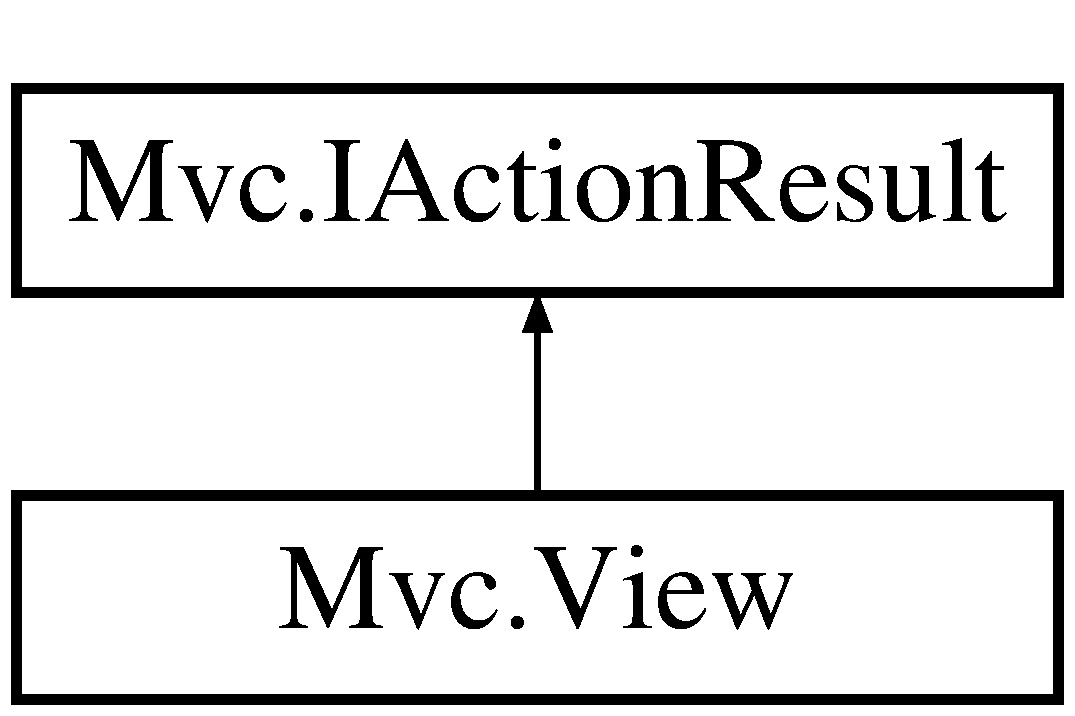
\includegraphics[height=2.000000cm]{class_mvc_1_1_view}
\end{center}
\end{figure}
\subsection*{Public Member Functions}
\begin{DoxyCompactItemize}
\item 
\hyperlink{class_mvc_1_1_view_a8a3cc05e4b1f355a5668970c7e633e85}{View} (string template, object data, int code, string physical\+Path, \hyperlink{class_mvc_1_1_route}{Route} route)
\begin{DoxyCompactList}\small\item\em Constructor of \hyperlink{class_mvc_1_1_view}{View} class \end{DoxyCompactList}\item 
int \hyperlink{class_mvc_1_1_view_a7e723a9bafb2f876175d1396c06da062}{Code} ()
\begin{DoxyCompactList}\small\item\em Gets the status code of the response. \end{DoxyCompactList}\item 
Memory\+Stream \hyperlink{class_mvc_1_1_view_a8a5a1a1990be0c3704b4f3262c503a2a}{Response} ()
\begin{DoxyCompactList}\small\item\em Gets the response of the controller in a stream. \end{DoxyCompactList}\item 
string \hyperlink{class_mvc_1_1_view_a0b14b3b8e85c97ada45a32dfcc30f157}{Content\+Type} ()
\begin{DoxyCompactList}\small\item\em Gets the content type of the response. \end{DoxyCompactList}\item 
string \hyperlink{class_mvc_1_1_view_a6628a16ae93e0269d91413a3a38d0132}{Redirection} ()
\begin{DoxyCompactList}\small\item\em Gets the url where the response is going to redirect (if there is any). \end{DoxyCompactList}\end{DoxyCompactItemize}


\subsection{Detailed Description}
Representative class of a custom view. 



Definition at line 14 of file View.\+cs.



\subsection{Constructor \& Destructor Documentation}
\mbox{\Hypertarget{class_mvc_1_1_view_a8a3cc05e4b1f355a5668970c7e633e85}\label{class_mvc_1_1_view_a8a3cc05e4b1f355a5668970c7e633e85}} 
\index{Mvc\+::\+View@{Mvc\+::\+View}!View@{View}}
\index{View@{View}!Mvc\+::\+View@{Mvc\+::\+View}}
\subsubsection{\texorpdfstring{View()}{View()}}
{\footnotesize\ttfamily Mvc.\+View.\+View (\begin{DoxyParamCaption}\item[{string}]{template,  }\item[{object}]{data,  }\item[{int}]{code,  }\item[{string}]{physical\+Path,  }\item[{\hyperlink{class_mvc_1_1_route}{Route}}]{route }\end{DoxyParamCaption})}



Constructor of \hyperlink{class_mvc_1_1_view}{View} class 


\begin{DoxyParams}{Parameters}
{\em template} & A string representing the name of the view template.\\
\hline
{\em data} & An object with the data to be passed to the view template.\\
\hline
{\em code} & An int representing the status code.\\
\hline
{\em physical\+Path} & A string representing the physical path of the App.\\
\hline
{\em route} & A \hyperlink{class_mvc_1_1_route}{Route} object representing the information of the route\\
\hline
\end{DoxyParams}


Definition at line 50 of file View.\+cs.



\subsection{Member Function Documentation}
\mbox{\Hypertarget{class_mvc_1_1_view_a7e723a9bafb2f876175d1396c06da062}\label{class_mvc_1_1_view_a7e723a9bafb2f876175d1396c06da062}} 
\index{Mvc\+::\+View@{Mvc\+::\+View}!Code@{Code}}
\index{Code@{Code}!Mvc\+::\+View@{Mvc\+::\+View}}
\subsubsection{\texorpdfstring{Code()}{Code()}}
{\footnotesize\ttfamily int Mvc.\+View.\+Code (\begin{DoxyParamCaption}{ }\end{DoxyParamCaption})}



Gets the status code of the response. 

\begin{DoxyReturn}{Returns}
An int representing the status code
\end{DoxyReturn}


Implements \hyperlink{interface_mvc_1_1_i_action_result_ab6b85ae50597587395df99b972c3d26b}{Mvc.\+I\+Action\+Result}.



Definition at line 63 of file View.\+cs.

\mbox{\Hypertarget{class_mvc_1_1_view_a0b14b3b8e85c97ada45a32dfcc30f157}\label{class_mvc_1_1_view_a0b14b3b8e85c97ada45a32dfcc30f157}} 
\index{Mvc\+::\+View@{Mvc\+::\+View}!Content\+Type@{Content\+Type}}
\index{Content\+Type@{Content\+Type}!Mvc\+::\+View@{Mvc\+::\+View}}
\subsubsection{\texorpdfstring{Content\+Type()}{ContentType()}}
{\footnotesize\ttfamily string Mvc.\+View.\+Content\+Type (\begin{DoxyParamCaption}{ }\end{DoxyParamCaption})}



Gets the content type of the response. 

\begin{DoxyReturn}{Returns}
A string representing the content type of the response
\end{DoxyReturn}


Implements \hyperlink{interface_mvc_1_1_i_action_result_a8ad08f29bba90dfbe06d7a00465af10a}{Mvc.\+I\+Action\+Result}.



Definition at line 84 of file View.\+cs.

\mbox{\Hypertarget{class_mvc_1_1_view_a6628a16ae93e0269d91413a3a38d0132}\label{class_mvc_1_1_view_a6628a16ae93e0269d91413a3a38d0132}} 
\index{Mvc\+::\+View@{Mvc\+::\+View}!Redirection@{Redirection}}
\index{Redirection@{Redirection}!Mvc\+::\+View@{Mvc\+::\+View}}
\subsubsection{\texorpdfstring{Redirection()}{Redirection()}}
{\footnotesize\ttfamily string Mvc.\+View.\+Redirection (\begin{DoxyParamCaption}{ }\end{DoxyParamCaption})}



Gets the url where the response is going to redirect (if there is any). 

\begin{DoxyReturn}{Returns}
A string representing the redirection url
\end{DoxyReturn}


Implements \hyperlink{interface_mvc_1_1_i_action_result_a036707da116ea300eae90e105b8d1ced}{Mvc.\+I\+Action\+Result}.



Definition at line 93 of file View.\+cs.

\mbox{\Hypertarget{class_mvc_1_1_view_a8a5a1a1990be0c3704b4f3262c503a2a}\label{class_mvc_1_1_view_a8a5a1a1990be0c3704b4f3262c503a2a}} 
\index{Mvc\+::\+View@{Mvc\+::\+View}!Response@{Response}}
\index{Response@{Response}!Mvc\+::\+View@{Mvc\+::\+View}}
\subsubsection{\texorpdfstring{Response()}{Response()}}
{\footnotesize\ttfamily Memory\+Stream Mvc.\+View.\+Response (\begin{DoxyParamCaption}{ }\end{DoxyParamCaption})}



Gets the response of the controller in a stream. 

\begin{DoxyReturn}{Returns}
Memory\+Stream that represents the response of the controller.
\end{DoxyReturn}


Implements \hyperlink{interface_mvc_1_1_i_action_result_a7cf7423071384c7b2bac75a5f4d6e25c}{Mvc.\+I\+Action\+Result}.



Definition at line 72 of file View.\+cs.



The documentation for this class was generated from the following file\+:\begin{DoxyCompactItemize}
\item 
C\+:/\+Users/dieguito12/\+Code/sharpener-\/framework/src/\+Mvc/View.\+cs\end{DoxyCompactItemize}

%--- End generated contents ---

% Index
\backmatter
\newpage
\phantomsection
\clearemptydoublepage
\addcontentsline{toc}{chapter}{Index}
\printindex

\end{document}
